\documentclass{article}
\usepackage[utf8]{inputenc}   % Pour les fichiers en UTF-8
\usepackage[french]{babel}
\usepackage{float}
\usepackage{xcolor}
\usepackage{listings}
\usepackage{lipsum} 
\usepackage{eso-pic}
\usepackage{tikz}
\usepackage{everypage}
\usepackage{subcaption}
\usepackage{fancyhdr}
\usepackage[absolute,overlay]{textpos}
\usepackage{fancyheadings}
\usepackage{lastpage}
\usepackage{eso-pic}
\usepackage[french]{babel}
\usepackage[hidelinks]{hyperref}
\usepackage{float}
\usepackage[utf8]{inputenc}
\usepackage{titlesec}
\usepackage{amsmath}
\usepackage{amssymb}
\usepackage{pifont}
\usepackage{pgfplots}
\pgfplotsset{compat=1.18}
\usepackage{amsmath}
\usepackage{amssymb}
\usepackage{siunitx}
\usepackage{tabularx} % à mettre dans le préambule
\usepackage{lastpage} % pour \pageref{LastPage}
\usepackage{hyperref}

% Définition du style VHDL
\lstdefinestyle{VHDLStyle}{
    language=VHDL,
    basicstyle=\ttfamily\small,      % police monospaced et taille petite
    keywordstyle=\color{blue}\bfseries, % mots-clés en bleu et gras
    commentstyle=\color{green!60!black}\itshape, % commentaires en vert italique
    stringstyle=\color{red},         % chaînes de caractères en rouge
    numbers=left,                    % numéros de lignes à gauche
    numberstyle=\tiny\color{gray},   % style des numéros
    stepnumber=1,                    
    numbersep=5pt,                   
    backgroundcolor=\color{gray!10}, % couleur de fond du code
    frame=single,                    % encadré autour du code
    rulecolor=\color{black},         
    breaklines=true,                 % retour à la ligne automatique
    breakatwhitespace=true,          
    tabsize=2,                       
    showstringspaces=false,          
    captionpos=b                     
}


\usepackage[a4paper, margin=3.2cm, top=3.5cm, bottom=4cm]{geometry}

% Modifier - par numéro du TP à rendre
\title{Rapport Intermediaire - Conception Circuit Numérique}
\author{Davy CLARK \& Nolan BUCHET}
\date{Septembre 2025}

\begin{document}

\maketitle

\begin{figure}[H]
    \centering
    
\includegraphics[width=1\linewidth]{Graphix/Polytech_Univ.png}
\end{figure}

\vspace{10pt}

\begin{center}
        {\Huge Recepteur de Transmission LIN}
\end{center}

\vspace{10pt}

\begin{figure}[H]
    \centering
    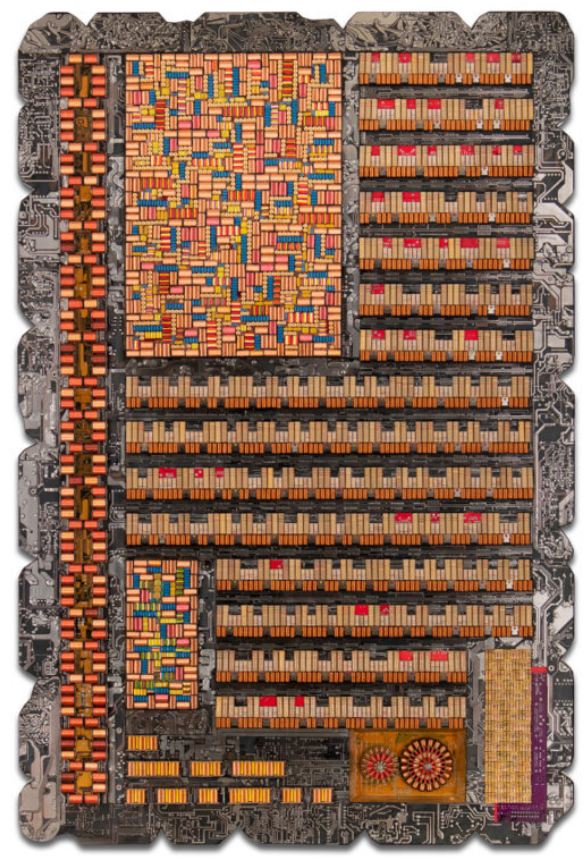
\includegraphics[width=0.4\linewidth]{Image_Base.png}
\end{figure}

\thispagestyle{empty} 

% LOGO IUT
\AddEverypageHook{%
  \begin{textblock*}{100cm}(100cm,100cm) % Ajustez les coordonnées pour décaler l'image
  \begin{tikzpicture}[remember picture, overlay]
    \node[anchor=north east, inner sep=18pt] at (current page.north east) {%
      
\includegraphics[scale=0.18]{Graphix/Logo_Universite_de_nantes.png}%
    };
  \end{tikzpicture}%
  \end{textblock*}
}

\AddEverypageHook{%
  \begin{textblock*}{100cm}(100cm,100cm) % Ajustez '15cm' pour déplacer l'image plus à droite
    \begin{tikzpicture}[remember picture, overlay]
      \node[anchor=north west, inner sep=25pt] at (current page.north west) {%
        
\includegraphics[scale=0.50]{Graphix/logo_poly.png}%
      };
    \end{tikzpicture}%
  \end{textblock*}
}



% NOM FICHIER
\AddEverypageHook{%
  \begin{textblock*}{1cm}(1cm,1cm)
  \end{textblock*}
  \begin{tikzpicture}[remember picture, overlay]
    \node[anchor=north, inner sep=50pt] at (current page.north) {%    
    {\fontsize{10}{13}\selectfont Compte Rendu Intermediaire Conception Circuit Numérique}
    };
  \end{tikzpicture}%
}

% PAGE
\AddEverypageHook{%
  \begin{textblock*}{1cm}(1cm,1cm)
  \end{textblock*}
  \begin{tikzpicture}[remember picture, overlay]
    \node[anchor=south, inner sep=50pt] at (current page.south) {%
    \thepage/\pageref{LastPage}
    };
  \end{tikzpicture}%
}

% NOM PRENOM
\AddEverypageHook{%
  \begin{textblock*}{1cm}(1cm,1cm)
  \end{textblock*}
  \begin{tikzpicture}[remember picture, overlay]
    \node[anchor=south west, inner sep=50pt] at (current page.south west) {%    
    {\fontsize{10}{13}\selectfont Davy CLARK \& Nolan BUCHET}
    };
  \end{tikzpicture}%
}

% DATE
\AddEverypageHook{%
  \begin{textblock*}{1cm}(1cm,1cm)
  \end{textblock*}
  \begin{tikzpicture}[remember picture, overlay]
    \node[anchor=south east, inner sep=50pt] at (current page.south east) {%    
    {\fontsize{10}{13}\selectfont Septembre 2025}
    };
  \end{tikzpicture}%
}


\pagestyle{empty}
\pagestyle{fancy}

\fancyhead[L]{\large} % Left side of the header (section title)
\fancyhead[R]{\large} % Right side of the header (page number)

% Footer configuration
\fancyfoot[C]{\large} % Centered text in the footer

\renewcommand{\headrulewidth}{1pt} % Header rule thickness
\renewcommand{\footrulewidth}{1pt} % Footer rule thickness
 % Stock pied de page

\tableofcontents

\section{Introduction}

Le projet réalisé dans le cadre de l'enseignement de Conception de Circuits numériques a pour 
objectif de développer des compétences essentielles à la conception de systèmes embarqués, 
notamment la mise au point d'un circuit utilisant un composant logique programmable.
\newline

L'architecture électronique d'un véhicule repose sur une organisation de calculateurs distribués. 
L'exemple retenu s'inspire du fonctionnement d'un calculateur embarqué dans la portière d'une 
automobile, chargé de la gestion des rétroviseurs et des vitres électriques.
\newline

Dans ce contexte, deux sous-ensembles sont distingués : 
\begin{itemize}
    \item un sous-ensemble de supervision, qui génère les commandes pour les moteurs des rétroviseurs et des vitres électriques,
    \item un sous-ensemble d'interface, assurant la communication entre le sous-ensemble de supervision et les autres calculateurs du véhicule.
\end{itemize}

Ce rapport se concentre exclusivement sur ce second sous-ensemble, l'interface microprocesseur, afin d'étudier son rôle et sa conception.

L'un des objectifs principaux est d'appréhender la conception du circuit via la méthode MCSE (Méthode de Conception de Systèmes Électroniques), en mettant l'accent sur les étapes de spécifications et de conception. Le déroulement du rapport suit la logique du diagramme en Y.

\begin{figure}[H]
    \centering
    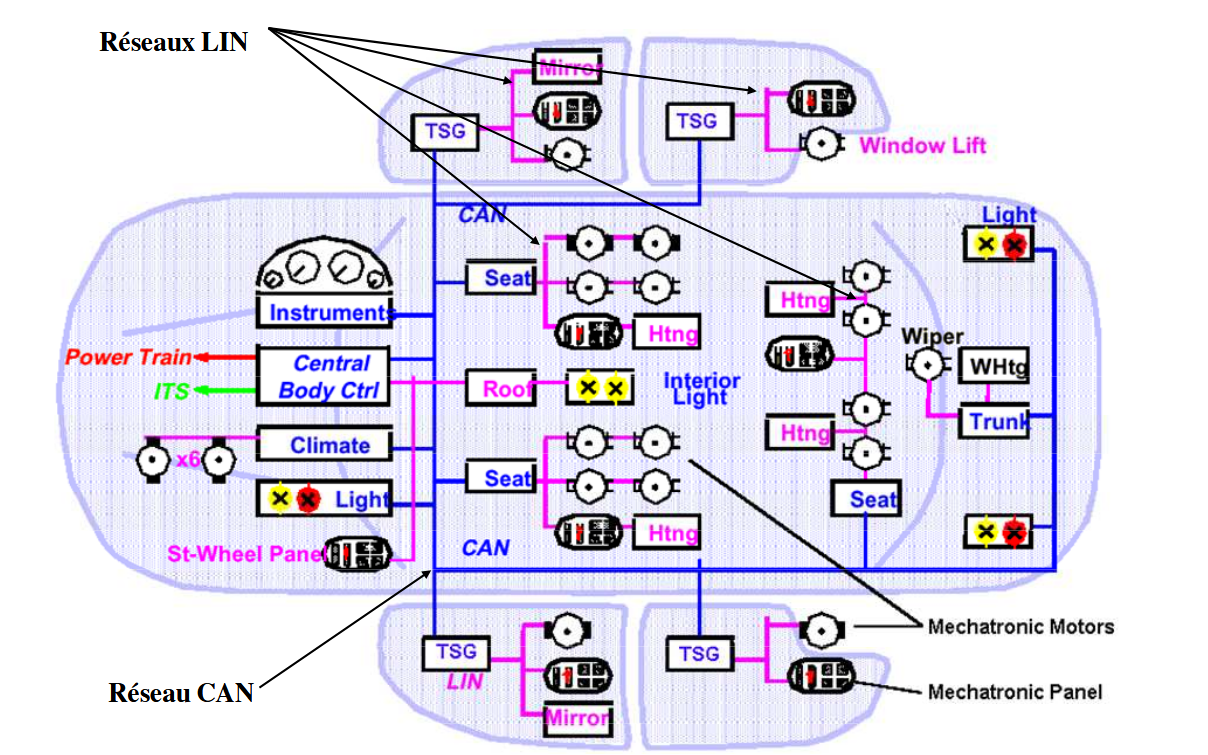
\includegraphics[width=0.8\linewidth]{images/Intro/Architecture_LIN.png}
    \caption{Exemple d'architecture d'un réseau dans un véhicule}
    \label{fig:placeholder}
\end{figure}

\section{Protocole LIN}

\subsubsection*{Architecture}  
Le bus LIN est un système \textit{mono-maître et multi-esclaves}. Un seul maître initie toutes les communications, ce qui rend inutile toute fonction d'arbitrage. Le nombre d'esclaves n'est pas limité par la norme mais dépend des contraintes électriques. L'architecture est dite \textit{flexible}, car on peut ajouter des nœuds esclaves sans modifier les nœuds existants.  

\begin{figure}[H]
    \centering
    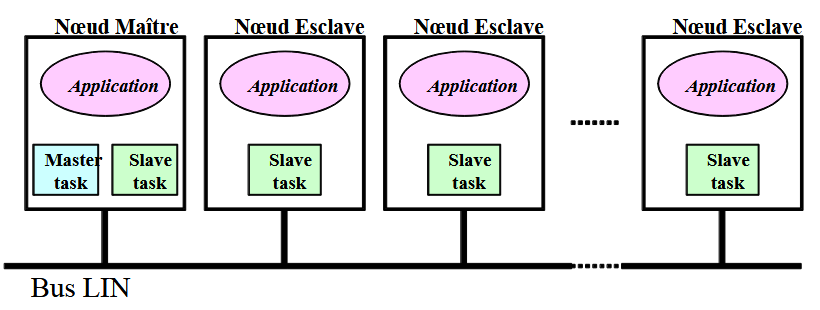
\includegraphics[width=0.8\linewidth]{images//Intro/Architecture_LIN_ME.png}
    \caption{Exemple d'architecture LIN}
    \label{fig:placeholder}
\end{figure}

\subsubsection*{Connexion}  
Le bus est constitué d'une \textit{seule ligne} reliée à chaque nœud par une sortie à collecteur ouvert. Le maître utilise une résistance de tirage de \SI{1}{k\ohm}, tandis que chaque esclave utilise \SI{30}{k\ohm}. La ligne est au niveau \textit{récessif (1)} lorsqu'aucun nœud ne force l'état, et au niveau \textit{dominant (0)} dès qu'au moins un nœud impose ce niveau.  

\begin{figure}[H]
    \centering
    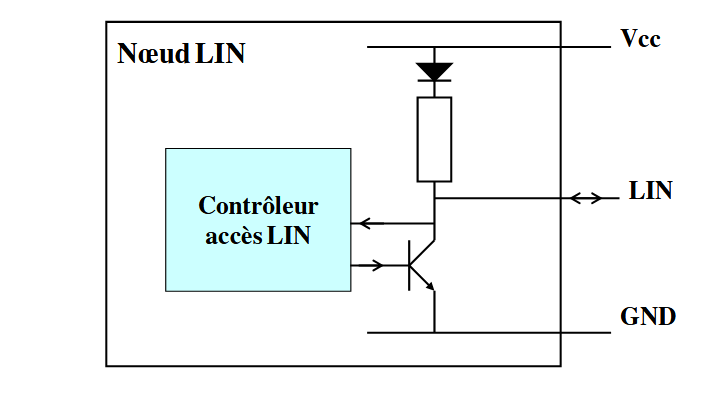
\includegraphics[width=0.5\linewidth]{images//Intro/Connection_LIN.png}
    \caption{Connexion physique d'un noeud à la ligne LIN}
    \label{fig:placeholder}
\end{figure}

\subsubsection*{Vitesse de transmission}  
Le débit varie de \SI{1}{kbit/s} à \SI{20}{kbit/s}, fixé pour une architecture donnée. Trois vitesses sont recommandées :  
\begin{itemize}
    \item \textbf{Lente} : 2400 bit/s,  
    \item \textbf{Moyenne} : 9600 bit/s,  
    \item \textbf{Rapide} : 19200 bit/s.  
\end{itemize}

\subsubsection*{Communications et trames}  
Les messages LIN sont composés de plusieurs champs :  
\begin{itemize}
    \item \textit{Synchronisation Break} : marque le début du message,  
    \item \textit{Synchronisation Field} : alignement des horloges (valeur 0x55),  
    \item \textit{Identification Field} : contenu et longueur des données, avec contrôle de parité,  
    \item \textit{Data Field} : octets d'information transmis du LSB vers le MSB,  
    \item \textit{Checksum Field} : somme de contrôle des données (modulo 256 inversée).  
\end{itemize}

\begin{figure}[H]
    \centering
    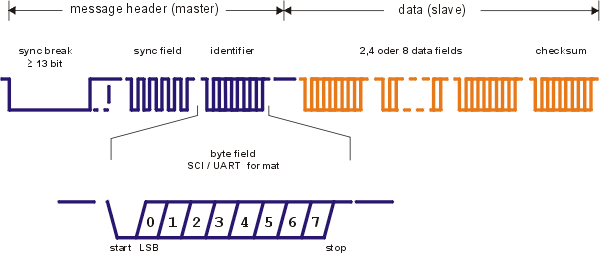
\includegraphics[width=0.8\linewidth]{images//Intro/Trame_LIN.png}
    \caption{Type de Trame Protocol LIN}
    \label{fig:placeholder}
\end{figure}

Une communication peut être de deux types :  
\begin{itemize}
    \item \textbf{Écriture} : le maître envoie l'intégralité du message,  
    \item \textbf{Lecture} : le maître envoie seulement l'entête, puis reçoit la réponse de l'esclave.  
\end{itemize}




\section{Cahier des Charges}

Le projet se concentre sur une partie restreinte du récepteur LIN, uniquement pour la réception de trames de type \textbf{« écriture »}, avec une \textbf{entrée LIN unique} et une vitesse fixée à \SI{19200}{bit/s}. La distinction maître/esclave et la connexion physique complète ne sont pas traitées.

\subsubsection*{Limitations et simplifications :}
\begin{itemize}
    \item Pas de gestion de perte d'octets,
    \item Vérification des bits start/stop par un seul échantillon,
    \item Pas de contrôle de parité ni de vérification du checksum.
\end{itemize}

\subsubsection*{Fonctionnalités attendues :}
\begin{itemize}
    \item Conversion série → parallèle (données de 8 bits) pour un microprocesseur,
    \item Possibilité de \textbf{filtrer les messages} grâce à un registre de comparaison \texttt{SelAdr} (8 bits),
    \item Signalisation de fin de réception (\texttt{M\_Received}) uniquement si l'identifiant reçu correspond à \texttt{SelAdr},
    \item Réinitialisation des compteurs et effacement des messages non valides.
\end{itemize}

\subsubsection*{Gestion des messages :}
\begin{itemize}
    \item Un seul message peut être stocké à la fois (FIFO),
    \item Les octets doivent être accessibles dans leur ordre d'arrivée, même si le message est encore en cours de réception,
    \item Tous les octets doivent être mémorisés, indépendamment du filtrage,
    \item Le récepteur doit déterminer la fin du message et l'indiquer au microprocesseur.
\end{itemize}

\subsubsection*{État du récepteur :}  
Accessible par registre ( ETAT ) à tout moment, il doit indiquer :
\begin{itemize}
    \item si un message a été reçu (après filtrage),
    \item le nombre d'octets reçus,
    \item les erreurs simples de réception (bits START/STOP, durée du \textit{synchro break}).
\end{itemize}

Après lecture du registre d'état, les champs sont réinitialisés (sauf le compteur d'octets reçus).

\subsubsection*{Contraintes supplémentaires :}
\begin{itemize}
    \item Interface physique avec le microprocesseur imposée,
    \item Caractéristiques fonctionnelles, physiques et temporelles définies,
    \item Temps d'échanges précisés pour assurer la compatibilité avec l'environnement.
\end{itemize}

\begin{figure}[H]
    \centering
    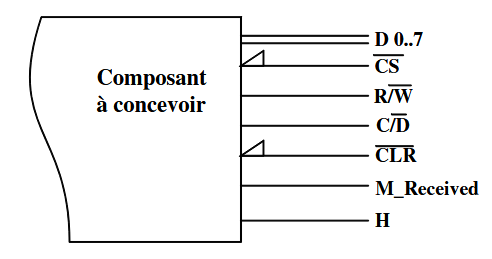
\includegraphics[width=0.8\linewidth]{images/CDC/Compo_concevoir.png}
    \caption{Interface microprocesseur associée au circuit à concevoir}
    \label{fig:placeholder}
\end{figure}

\begin{figure}[H]
    \centering
    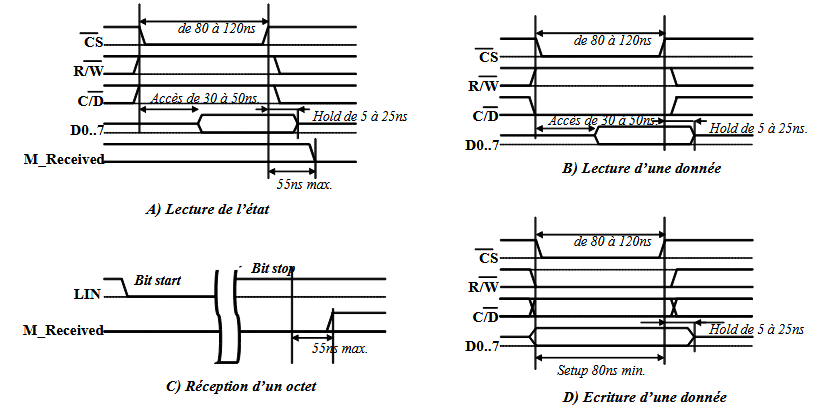
\includegraphics[width=0.8\linewidth]{images/CDC/Chrono.png}
    \caption{Chronogrammes des échanges entre le circuit et son environnement}
    \label{fig:placeholder}
\end{figure}

% Page 2 TD DAVY
\begin{figure}[H]
    \centering
    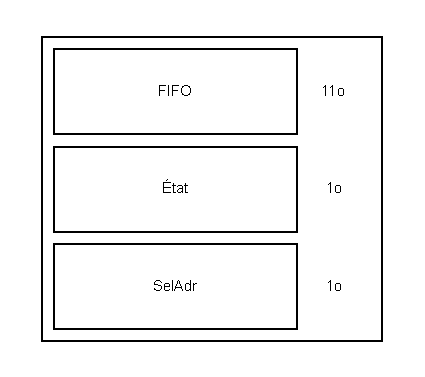
\includegraphics[width=0.8\linewidth]{images/CDC/Schema_Fifi_etat.pdf}
    \caption{Schema Conception Registre interne Système}
    \label{fig:placeholder}
\end{figure}



\section{Description des différentes spécifications définies en travaux dirigés}

\subsection*{Objectif}

Les spécifications ont pour objectif de définir le comportement attendu du système, c’est-à-dire 
\textbf{ce que le circuit doit faire} en réponse au cahier des charges. 
Elles constituent une description \textbf{fonctionnelle} du système, exprimée du point de vue de son 
\textbf{environnement} — c’est-à-dire de tout ce qui interagit avec lui, sans se soucier de son 
implémentation interne.

\medskip

Cette phase correspond au \textbf{niveau de spécification fonctionnelle} dans le diagramme en Y. 
Elle adopte une approche \textbf{boîte noire}, centrée sur les entrées et sorties observables, 
indépendamment de toute considération technologique (langage, type logique, fréquence, etc.).

\medskip

Le cahier des charges indique que le circuit doit pouvoir \textbf{communiquer à la fois avec le système 
de trame LIN et avec un microcontrôleur}. 
Afin de clarifier les fonctions du système, nous avons choisi de le \textbf{décomposer en deux sous-blocs principaux} :
\begin{itemize}
    \item un bloc de \textbf{réception de trame LIN}, chargé de décoder et de stocker les données reçues ;
    \item un bloc d’\textbf{interface microprocesseur}, permettant l’échange de données et de signaux de contrôle avec le microcontrôleur.
\end{itemize}

\begin{figure}[H]
   \centering
   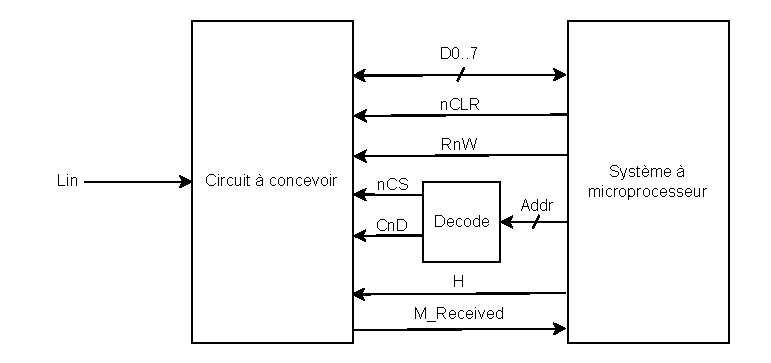
\includegraphics[width=0.8\linewidth]{images/CDC/Schema_cdc_final.pdf}
   \caption{Description fonctionnelle du circuit à concevoir}
   \label{fig:placeholder}
\end{figure}

\subsection{Interface Microprocesseur}

Ce sous-système permet la communication entre le circuit et le microprocesseur.  
Les signaux décrits ici représentent les \textbf{flux d’informations échangés} (données, commandes, synchronisation, validation), 
sans spécifier leur codage logique ni leur type de signal électrique.

\begin{center}
\renewcommand{\arraystretch}{1.2}
\small
\begin{tabularx}{\textwidth}{|c||c|c|X|}
    \hline			
    \textbf{Signal} & \textbf{Sens} & \textbf{Nature} & \textbf{Rôle fonctionnel}  \\ \hline 
    D\_BUS & Bidirectionnel & Données & Bus de transfert de données entre le microprocesseur et le circuit \\ 
    CS & Entrée & Commande & Sélection du circuit (validation de la communication) \\ 
    RW & Entrée & Commande & Indique une opération de lecture ou d’écriture \\ 
    CD & Entrée & Commande & Sélectionne entre registre de commande et registre de données \\ 
    RESET & Entrée & Commande & Réinitialisation du système \\ 
    MSG\_RECEIVED & Sortie & Indicateur & Signal indiquant la fin de réception d’une trame \\ 
    CLK & Entrée & Synchronisation & Signal d’horloge du système \\ 
    \hline  
\end{tabularx}
\end{center}

\subsection{Bloc Réception de Trame LIN}

Ce bloc assure le \textbf{décodage séquentiel} des trames LIN reçues.  
Il analyse le flux série provenant du bus LIN et extrait les octets de données en respectant la structure du protocole.

\begin{center}
\renewcommand{\arraystretch}{1.2}
\small
\begin{tabularx}{\textwidth}{|c||c|c|X|}
    \hline			
    \textbf{Signal} & \textbf{Sens} & \textbf{Nature} & \textbf{Rôle fonctionnel}  \\ \hline 
    LIN\_RX & Entrée & Données & Flux série reçu depuis le bus LIN \\ 
    DATA\_OUT & Sortie & Données & Octet de données extrait et validé \\ 
    VALID & Sortie & Indicateur & Indique la disponibilité d’un nouvel octet reçu \\ 
    \hline  
\end{tabularx}
\end{center}

\subsection{Mémoire FIFO}

Ce bloc a pour rôle de \textbf{stocker temporairement les octets reçus} avant leur transfert vers le microprocesseur.  
Il fonctionne selon le principe « premier entré, premier sorti ».

\begin{center}
\renewcommand{\arraystretch}{1.2}
\small
\begin{tabularx}{\textwidth}{|c||c|c|X|}
    \hline
    \textbf{Signal} & \textbf{Sens} & \textbf{Nature} & \textbf{Rôle fonctionnel} \\ \hline
    DATA\_IN & Entrée & Données & Octet à mémoriser dans la file FIFO \\ 
    DATA\_OUT & Sortie & Données & Octet extrait de la file FIFO \\ 
    WRITE\_REQ & Entrée & Commande & Requête d’écriture (nouvelle donnée reçue) \\ 
    READ\_REQ & Entrée & Commande & Requête de lecture (demande du microprocesseur) \\ 
    EMPTY & Sortie & Indicateur & Indique que la FIFO est vide \\ 
    FULL & Sortie & Indicateur & Indique que la FIFO est pleine \\ 
    \hline
\end{tabularx}
\end{center}

\subsection{Registre d’État}

Le registre d’état fournit une \textbf{synthèse du déroulement de la réception}.  
Il conserve les informations nécessaires à la supervision ou au diagnostic 
(erreurs détectées, nombre d’octets reçus, trame complète, etc.).

\begin{center}
\renewcommand{\arraystretch}{1.2}
\small
\begin{tabularx}{\textwidth}{|c||c|c|X|}
    \hline			
    \textbf{Signal} & \textbf{Sens} & \textbf{Nature} & \textbf{Rôle fonctionnel}  \\ \hline 
    ERR\_START & Entrée & Indicateur & Erreur sur le bit de début de trame \\ 
    ERR\_STOP & Entrée & Indicateur & Erreur sur le bit de fin de trame \\ 
    ERR\_SYNC & Entrée & Indicateur & Erreur de synchronisation \\ 
    BYTE\_COUNT & Entrée & Données & Nombre d’octets reçus dans la trame \\ 
    FRAME\_VALID & Entrée & Indicateur & Validation de la réception complète \\ 
    STATE\_OUT & Sortie & Données & Octet d’état global de la réception \\ 
    \hline  
\end{tabularx}
\end{center}


\section{Description et justification de la structure fonctionnelle}

\subsubsection*{Objectifs}

Cette section présente l'organisation du système en blocs fonctionnels et décrit leurs 
interactions. Chaque bloc (réception de trame, FIFO, registre d'état, interface microprocesseur) 
est expliqué dans son rôle et sa contribution au fonctionnement global. L'objectif est de montrer 
comment les fonctionnalités spécifiées sont réparties de manière logique pour répondre au cahier 
des charges.
\newline

Dans cette section, nous établissons une structure fonctionnelle indépendante de la technologie.

\begin{figure}[H]
    \centering
    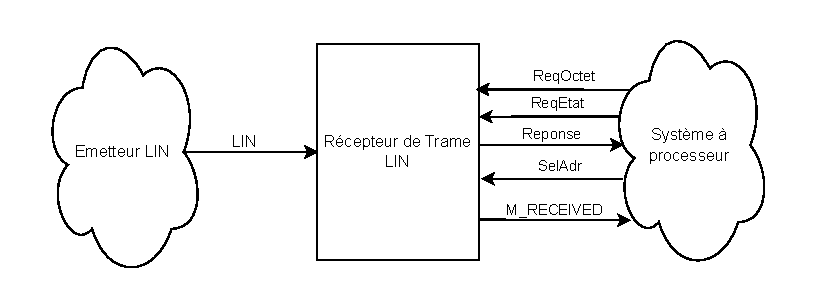
\includegraphics[width=0.8\linewidth]{images/inter/Structure_Fonc_Circuit.pdf}
    \caption{Structure fonctionnelle du système}
    \label{fig:placeholder}
\end{figure}

Pour le moment, nous nous sommes limités à deux blocs principaux : l'interface microprocesseur et 
la réception des trames. Ces deux blocs sont connectés à un bloc d'échange, qui permet la 
communication entre eux. Ce bloc assure l'interprétation des échanges avec le microprocesseur ainsi 
que la gestion des deux registres de données.
\newline

% page 12
\begin{figure}[H]
    \centering
    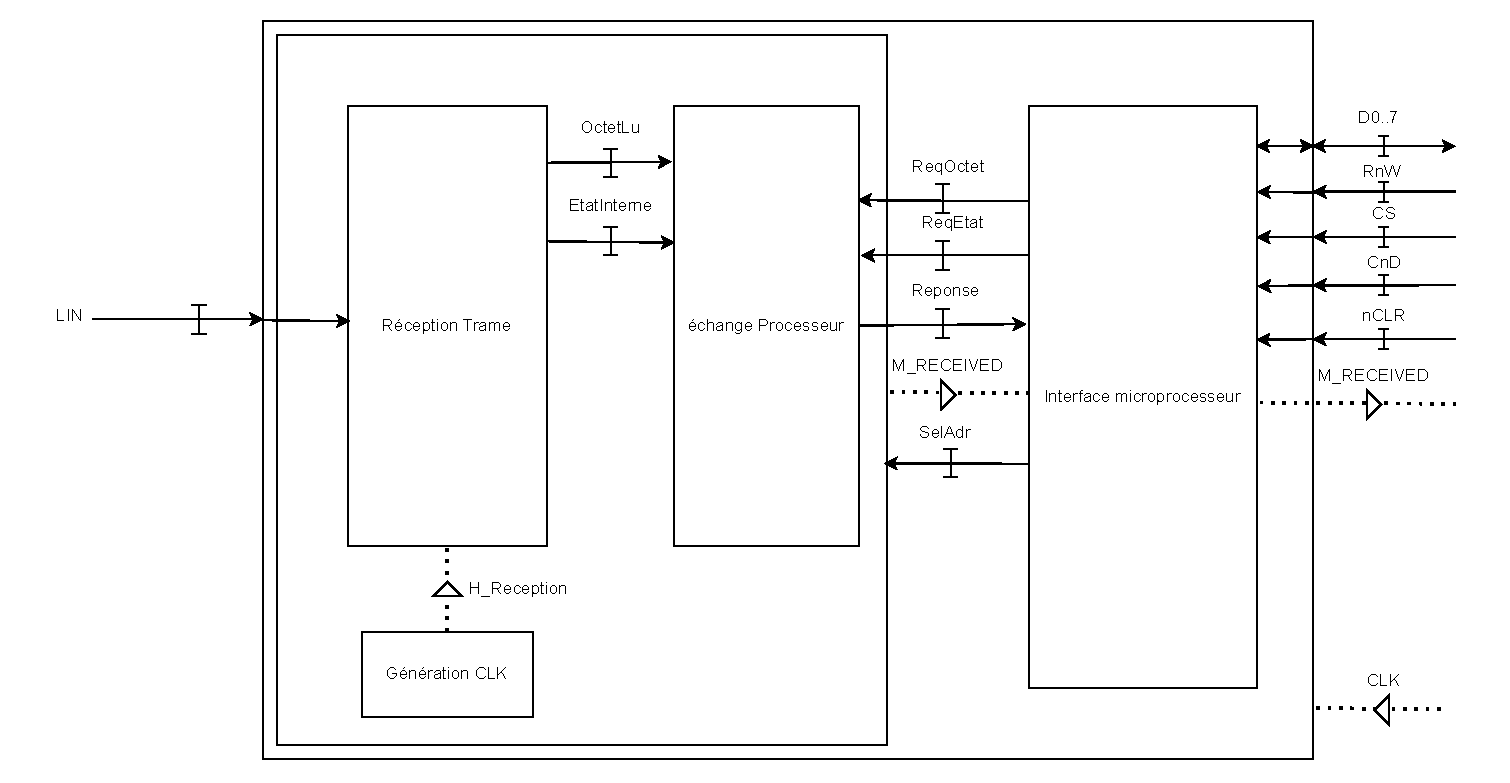
\includegraphics[width=0.8\linewidth]{images/inter/Schema_base_circuit.pdf}
    \caption{Architecture du système de réception de trame LIN V1}
    \label{fig:placeholder}
\end{figure}

Nous pouvons également représenter l'automate du système de communication avec le processeur : 

\begin{figure}[H]
    \centering
    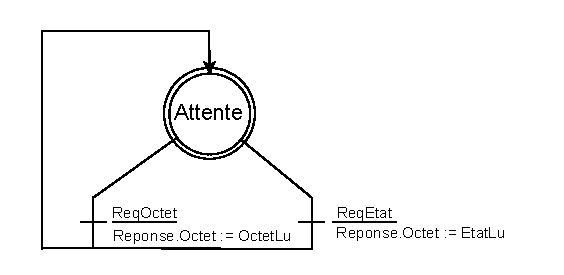
\includegraphics[width=0.8\linewidth]{images/inter/Echange_Processeur.pdf}
    \caption{Échanges avec le processeur}
    \label{fig:placeholder}
\end{figure}


Dans notre démarche d'optimisation du système, nous nous sommes rendu compte que le bloc d'échange 
microprocesseur pouvait être intégré au bloc d'interface. Cela permettra de supprimer des signaux 
supplémentaires, inutiles et encombrants.
\newline

%page 13
\begin{figure}[H]
    \centering
    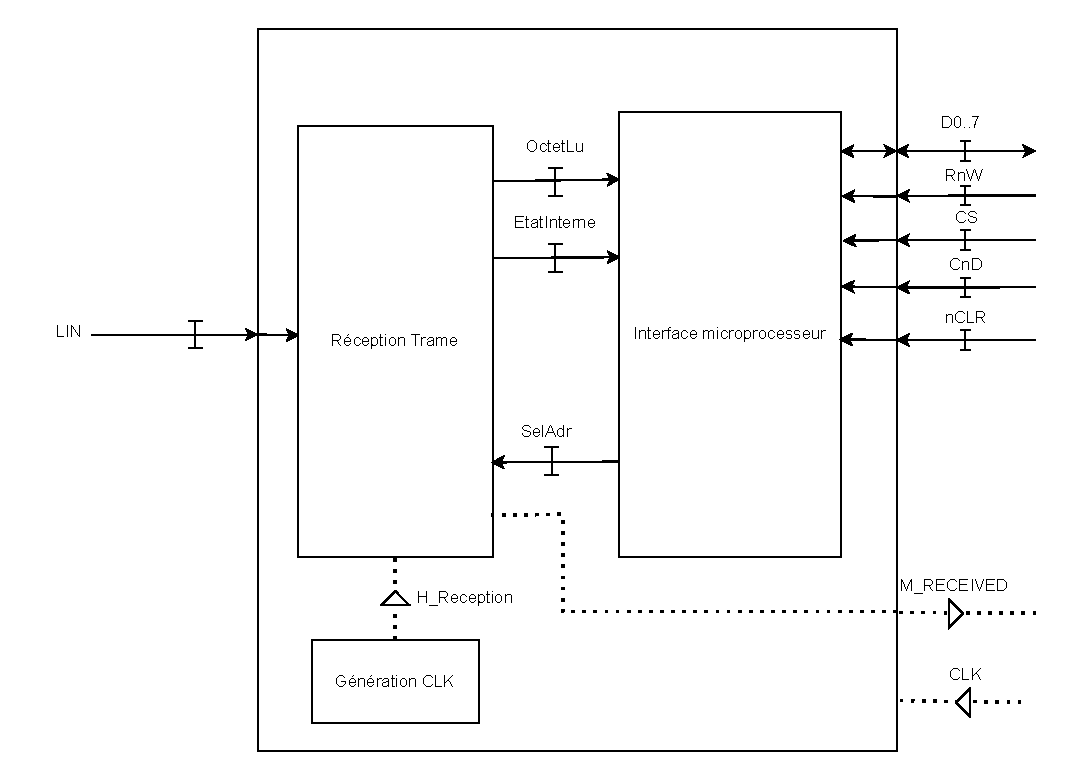
\includegraphics[width=0.8\linewidth]{images/inter/Schema_avance_circuit.pdf}
    \caption{Architecture du système de réception de trame LIN V2}
    \label{fig:placeholder}
\end{figure}

Par la suite, nous avons décidé d'ajouter deux blocs de registres internes : le registre de stockage 
des données de la trame LIN (FIFO) et le registre d'état interne (ETAT), qui permet de connaître les 
informations sur l'état de la réception.
\newline

%page 16
\begin{figure}[H]
    \centering
    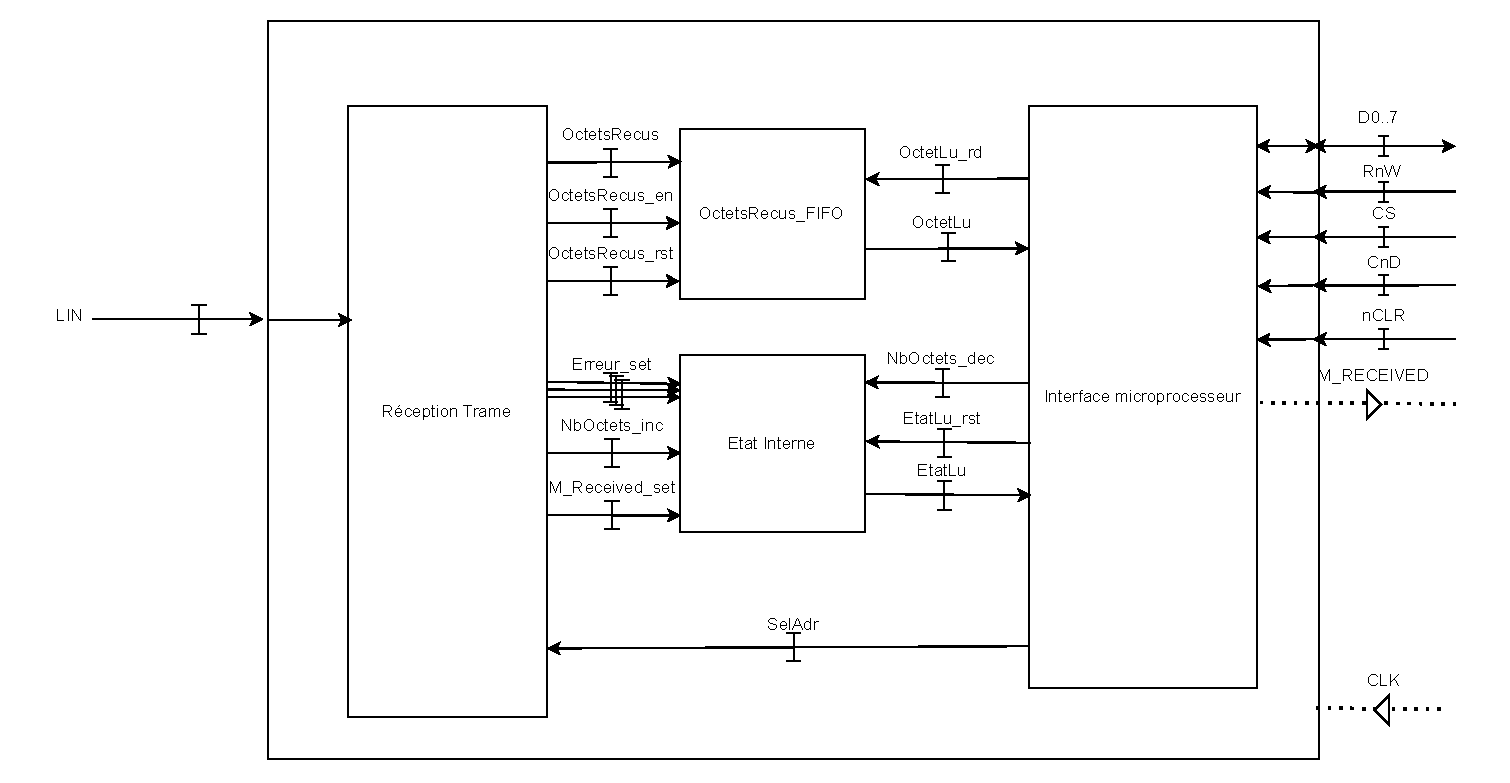
\includegraphics[width=0.8\linewidth]{images/inter/Schema_Final.pdf}
    \caption{Description finale du circuit}
    \label{fig:placeholder}
\end{figure}

Comme indiqué ci-dessus, dans le schéma de notre système global, nous avons décidé d'ajouter 
certains signaux internes entre les blocs de registres et les interfaces.
\newline

\subsubsection*{FIFO}

\begin{center}
\renewcommand{\arraystretch}{1.2} % espace vertical
\small % pour uniformiser la taille du texte
    \begin{tabularx}{\textwidth}{|c||c|c|X|}
     \hline			
       \textbf{Signaux} & \textbf{Mode} & \textbf{Type} & \textbf{Description}  \\ \hline 
       OctetRecu\_WR & IN & \texttt{STD\_LOGIC} & Read / Write opération \\
       OctetRecu\_RST & IN & \texttt{STD\_LOGIC} & Réinitialisation des données reçue \\
       OctetLu\_RD & IN & \texttt{STD\_LOGIC} & Sélection de la mémoire (Control / Data) \\
     \hline  
    \end{tabularx}
\end{center}

La définition de ces nouveaux signaux permet de gérer de manière précise le fonctionnement de la 
FIFO. OctetRecu\_WR est un signal d'écriture qui déclenche l'enregistrement d'un octet reçu dans 
la mémoire FIFO, garantissant que chaque donnée entrante est correctement stockée. OctetRecu\_RST 
est un signal de réinitialisation qui vide complètement la FIFO et remet à zéro tous les compteurs 
internes, permettant ainsi de reprendre la réception de données sans risque de corruption ou de 
chevauchement. OctetLu\_RD est un signal de lecture qui active l'accès aux données stockées dans 
la FIFO et permet leur transfert vers le microprocesseur ou d'autres blocs du système. Ensemble, 
ces signaux assurent une communication fiable, synchronisée et organisée entre l'interface 
microprocesseur et le registre de réception, tout en facilitant la gestion des flux de données 
entrants.
\newline

\subsubsection*{ETAT}

\begin{center}
\renewcommand{\arraystretch}{1.2} % espace vertical
\small % pour uniformiser la taille du texte
    \begin{tabularx}{\textwidth}{|c||c|c|X|}
     \hline			
       \textbf{Signaux} & \textbf{Mode} & \textbf{Type} & \textbf{Description}  \\ \hline 
       NbOctetRecu\_RST & IN & \texttt{STD\_LOGIC} & Réinitialisation du compteur d'octets \\
       DecNbOctet & IN & \texttt{STD\_LOGIC} & Flag de lecture pour FIFO \\
       EtatLu\_RST & IN & \texttt{STD\_LOGIC} & Reset de l'état lu \\
     \hline  
    \end{tabularx}
\end{center}

La définition de ces signaux du bloc ETAT permet de contrôler et de suivre l'état interne de la 
réception des données. NbOctetRecu\_RST réinitialise le compteur d'octets reçus, assurant un 
suivi précis du nombre de données traitées. DecNbOctet agit comme un indicateur de lecture pour 
la FIFO, signalant quand un octet peut être lu et transféré, ce qui permet une gestion correcte 
des flux de données. EtatLu\_RST permet de réinitialiser les informations d'état lues, garantissant 
que le système dispose toujours d'une représentation exacte de l'état actuel de la réception. 
Ensemble, ces signaux assurent une supervision fiable et synchronisée des opérations internes, 
facilitant le contrôle et la gestion du flux de données dans le système.


\section{Description et justification de la solution architecturale obtenue pour le circuit}

\subsubsection*{Objectifs}

Une fois la description fonctionnelle définie, la conception passe au \textbf{niveau architectural} du diagramme en Y.  
Cette phase vise à transformer la description fonctionnelle en une organisation interne du système : 
elle introduit les interfaces physiques, identifie les ressources de stockage et de traitement, et 
établit les principes de commande et de transfert des données.

\medskip

Cette description reste indépendante de la technologie d’implémentation (langage HDL, logique, FPGA, etc.) 
mais tient compte des contraintes structurelles et temporelles du système.  
Elle correspond au \textbf{niveau Registre-Transfert (RT)}.

\begin{itemize}
    \item Introduction et définition des interfaces physiques
    \item Identification des ressources logiques (registres, compteurs, opérateurs)
    \item Organisation structurelle du circuit au niveau RT
    \item Description du comportement séquentiel et des signaux de commande
\end{itemize}

\vspace{1em}

\subsection{Horloge}

La gestion de l’horloge constitue un élément fondamental de la synchronisation interne du système.

Le rapport entre la période du bit LIN et celle du processeur est défini par :

\[
N = \frac{T_{\text{bit}}}{T_{\text{processeur}}}
\]

Dans notre cas, le cahier des charges spécifie un cycle de lecture/écriture moyen de 100~ns et une vitesse de transmission de 19\,200~bit/s, soit :

\[
N = \frac{52~\mu s}{100~ns} = 520
\]

Pour notre implémentation, nous choisissons \(N = 2048\), une valeur supérieure qui facilite la synchronisation interne et la gestion des transitions logiques.

\subsection{Architecture de la Réception de Trame}

Ce bloc correspond à la partie du système chargée de la réception et du décodage des trames LIN.

\begin{center}
\renewcommand{\arraystretch}{1.2}
\small
\begin{tabularx}{\textwidth}{|c||c|c|X|}
\hline
\textbf{Signal} & \textbf{Sens} & \textbf{Nature} & \textbf{Rôle fonctionnel} \\ \hline
LIN & Entrée & Données & Signal série reçu depuis le bus LIN \\ 
SEL\_ADR & Entrée & Données & Sélection de l’adresse du composant \\ 
DATA\_OUT & Sortie & Données & Octet de données reçu \\ 
DATA\_WR & Sortie & Commande & Validation d’écriture vers la mémoire FIFO \\ 
DATA\_RST & Sortie & Commande & Réinitialisation des données reçues \\ 
ERR\_START & Sortie & Indicateur & Erreur sur bit de start \\ 
ERR\_STOP & Sortie & Indicateur & Erreur sur bit de stop \\ 
ERR\_SYNC & Sortie & Indicateur & Erreur de synchronisation (Synchro Break) \\ 
INC\_COUNT & Sortie & Commande & Incrémentation du compteur d’octets reçus \\ 
FRAME\_VALID & Sortie & Indicateur & Trame reçue et validée \\ 
COUNT\_RST & Sortie & Commande & Réinitialisation du compteur d’octets \\ 
\hline
\end{tabularx}
\end{center}

\medskip

Le bloc de réception repose sur une \textbf{machine séquentielle} structurée en deux sous-parties :
\begin{itemize}
    \item une \textbf{unité opérative} regroupant les registres, compteurs et multiplexeurs ;
    \item une \textbf{unité de commande} gérant la séquence d’opérations et les signaux de contrôle.
\end{itemize}

\begin{figure}[H]
    \centering
    \includegraphics[width=0.8\linewidth]{images/inter/Machine_Seq_Reception_trame.pdf}
    \caption{Organisation séquentielle du bloc de réception de trame}
    \label{fig:reception_seq}
\end{figure}

Les principales variables internes assurent la gestion du comptage, du stockage et du décalage des bits reçus :

\begin{table}[h!]
    \centering
    \resizebox{\textwidth}{!}{%
        \begin{tabular}{|c|c|c|c|c|}
            \hline
            \textbf{Variable} & \textbf{Taille (bit)} & \textbf{Opération} & \textbf{Opérateur} & \textbf{Signaux de contrôle} \\ 
            \hline
            n & $\log_2(N)$ & décrémentation, initialisation à $N-1$ ou $N/2$ & décompteur, Mux & n\_Load, n\_En, n\_select \\ 
            \hline
            NbTbit & 4 & décrémentation, initialisation à 13 ou 8 & décompteur, Mux & NBTbit\_Load, NBTbit\_en, NBTbit\_select \\ 
            \hline
            Identifier & 8 & sauvegarde & registre 8 bits & Identifier\_en \\ 
            \hline
            OctetsReçus & 8 & décalage bit à bit & registre à décalage & OctetReçu\_en \\ 
            \hline
            NbDataField & 3 & décrémentation, initialisation à 1, 3 ou 7 & décompteur, décodeur & NBdatafield\_en, NBdatafield\_load \\ 
            \hline
        \end{tabular}%
    }
\end{table}



\begin{figure}[H]
    \centering
    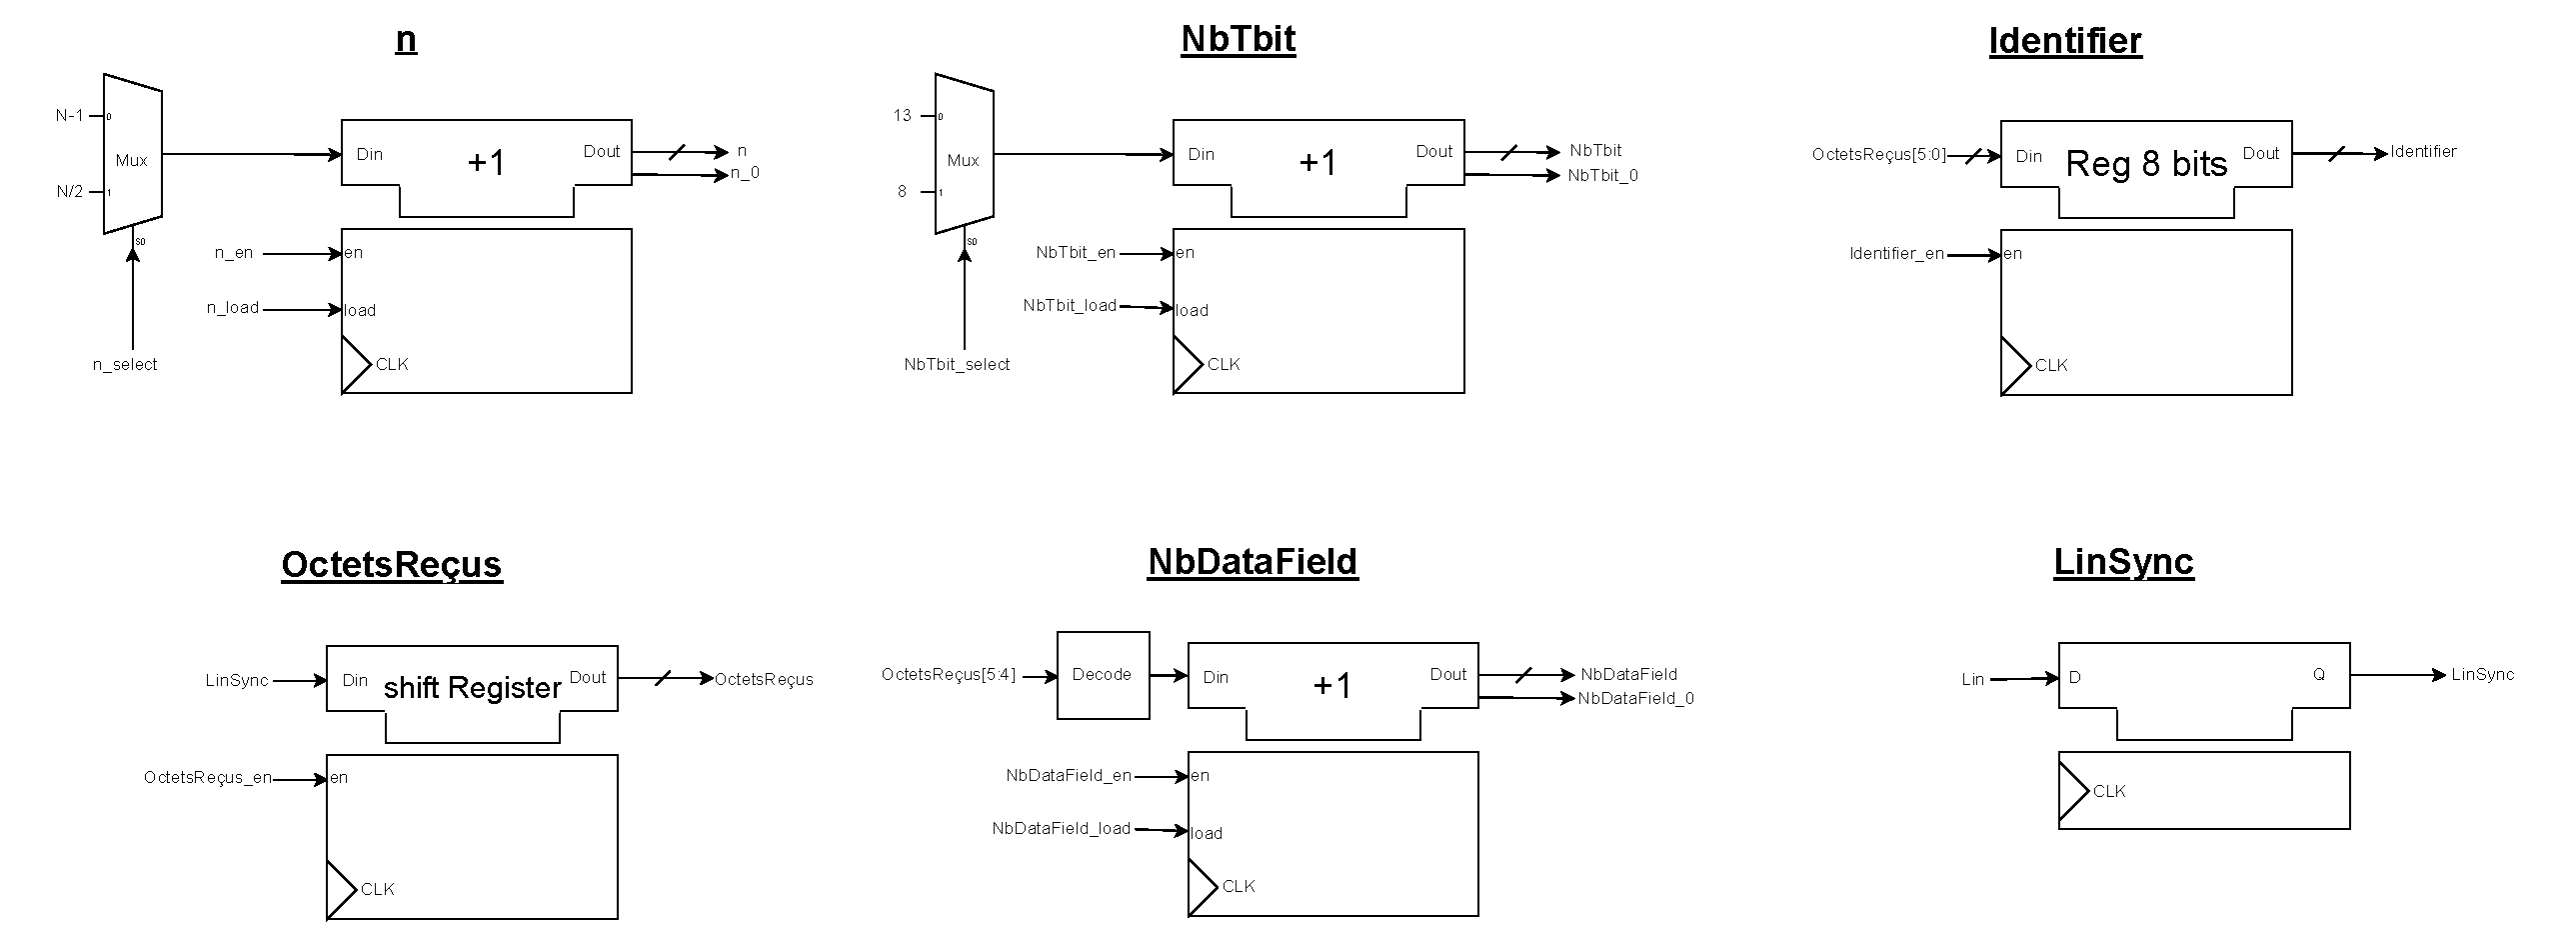
\includegraphics[width=0.95\linewidth]{images/inter/Structure_Reception_trame.pdf}
    \caption{Structure opérative du bloc de réception de trame}
    \label{fig:reception_structure}
\end{figure}

La partie commande est implémentée sous forme d’un \textbf{automate séquentiel}, représentant les différents états de réception d’une trame LIN.

\begin{figure}[H]
    \centering
    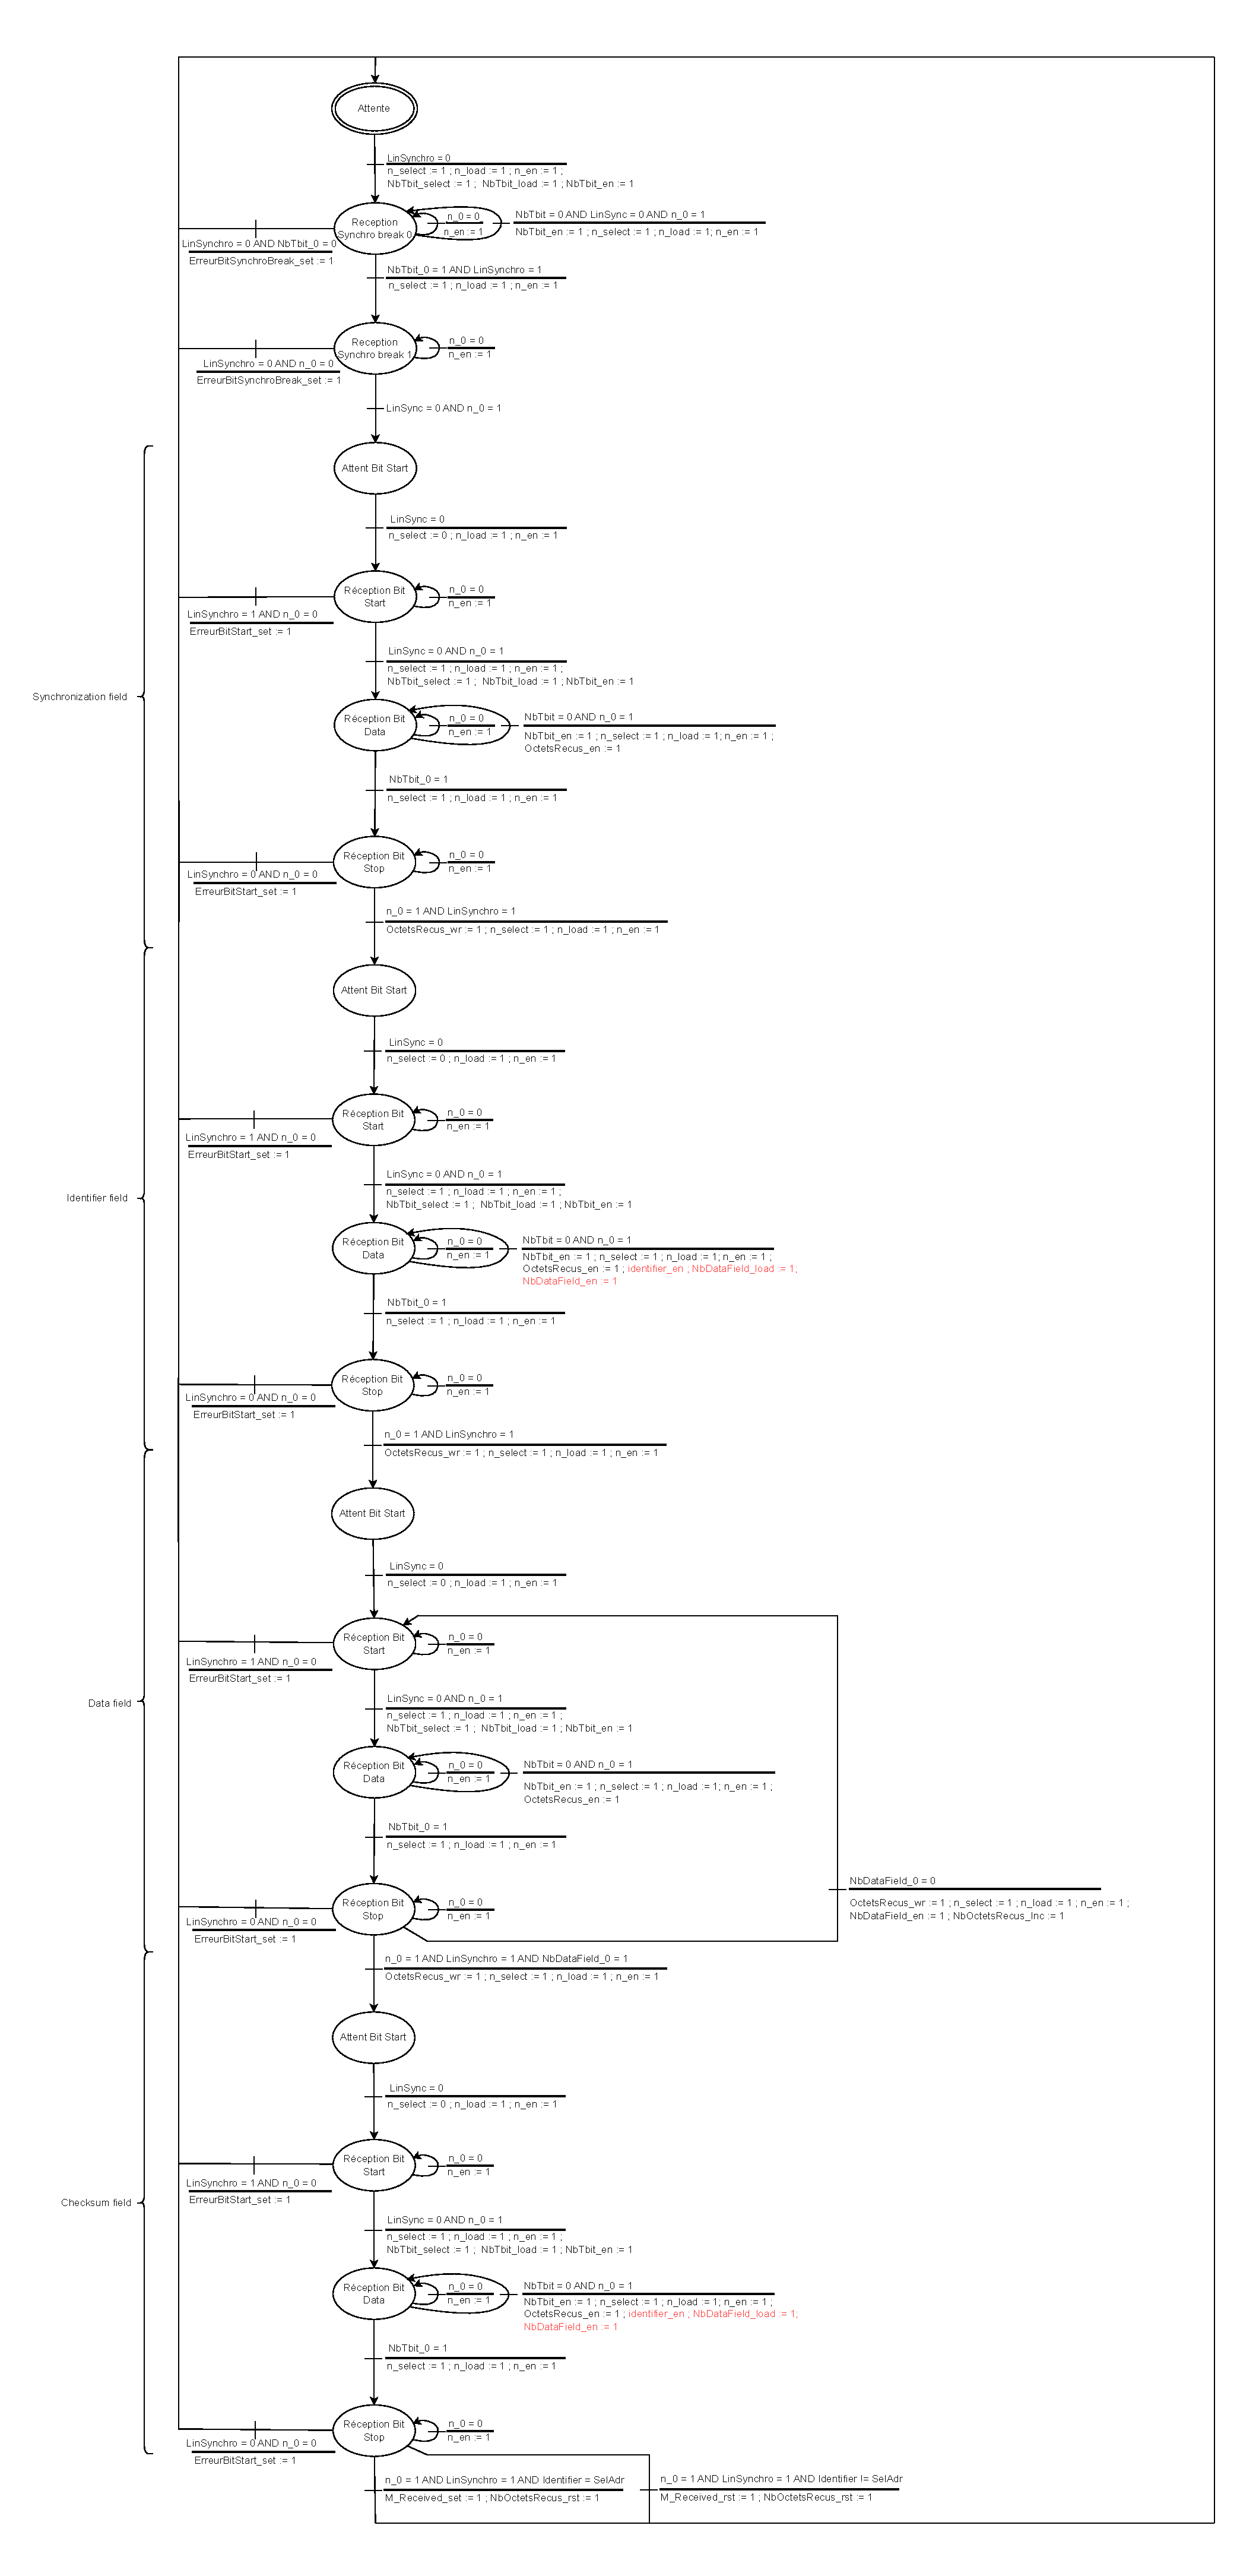
\includegraphics[width=0.6\linewidth]{images/inter/Automate_Reception_trame.pdf}
    \caption{Automate de réception de trame LIN}
    \label{fig:automate_reception}
\end{figure}

\subsection*{Description de l’automate}

L’automate décrit la séquence d’opérations depuis l’attente du signal de début jusqu’à la validation de la trame complète.  
Il gère successivement les phases suivantes :
\begin{itemize}
    \item \textbf{Attente et détection de break de synchronisation}
    \item \textbf{Réception du champ de synchronisation}
    \item \textbf{Réception de l’identifiant et des données}
    \item \textbf{Vérification du checksum et validation de la trame}
\end{itemize}

Les erreurs de synchronisation ou de bits sont détectées via des indicateurs spécifiques (erreurs de start, stop, ou synchro).  
Ce fonctionnement correspond à une \textbf{machine de Mealy}, dans laquelle les sorties dépendent à la fois des états internes et des entrées instantanées.

\begin{figure}[H]
    \centering
    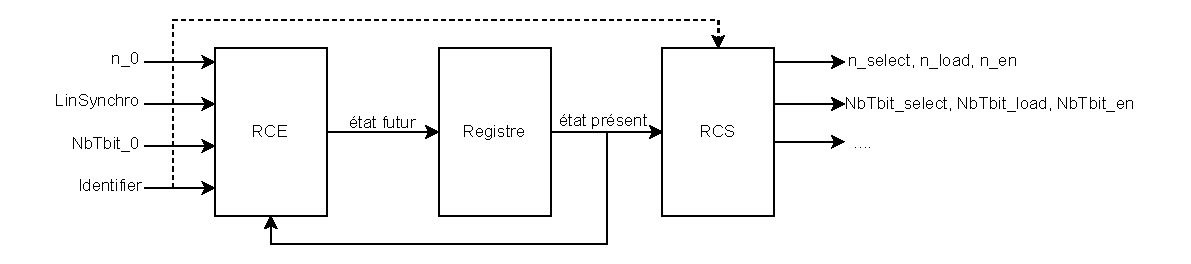
\includegraphics[width=0.8\linewidth]{images/inter/MEALY_Reception_trame.pdf}
    \caption{Machine de Mealy – Unité de commande de réception de trame}
    \label{fig:mealy_reception}
\end{figure}

\subsection{Architecture de l’Interface Microprocesseur}

Ce bloc gère les échanges entre le microprocesseur et les registres internes du système.  
Il coordonne la lecture et l’écriture des données, ainsi que la signalisation de fin de réception.

\begin{center}
\renewcommand{\arraystretch}{1.2}
\small
\begin{tabularx}{\textwidth}{|c||c|c|X|}
\hline
\textbf{Signal} & \textbf{Sens} & \textbf{Nature} & \textbf{Rôle fonctionnel} \\ \hline
D\_BUS & Bidirectionnel & Données & Bus de communication principal \\ 
CS & Entrée & Commande & Sélection du circuit \\ 
RW & Entrée & Commande & Lecture ou écriture \\ 
CD & Entrée & Commande & Sélection entre commande et données \\ 
RESET & Entrée & Commande & Réinitialisation du système \\ 
FRAME\_RECEIVED & Sortie & Indicateur & Signal de fin de réception \\ 
CLK & Entrée & Synchronisation & Horloge du système \\ 
STATE\_IN & Entrée & Données & État interne du système \\ 
DEC\_COUNT & Sortie & Commande & Décrémentation du compteur FIFO \\ 
STATE\_RST & Sortie & Commande & Réinitialisation de l’état \\ 
DATA\_IN & Entrée & Données & Donnée issue de la FIFO \\ 
DATA\_SEL & Sortie & Commande & Sélection du type de donnée affichée \\ 
\hline
\end{tabularx}
\end{center}

\begin{figure}[H]
    \centering
    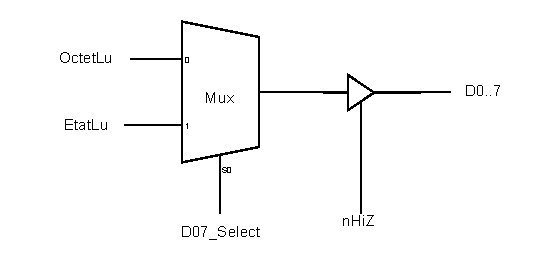
\includegraphics[width=0.8\linewidth]{images/inter/Structure_Interface_Micro.pdf}
    \caption{Structure opérative de l’interface microprocesseur}
    \label{fig:micro_interface}
\end{figure}

L’unité de commande correspondante est également décrite par un automate de type Mealy :

\begin{figure}[H]
    \centering
    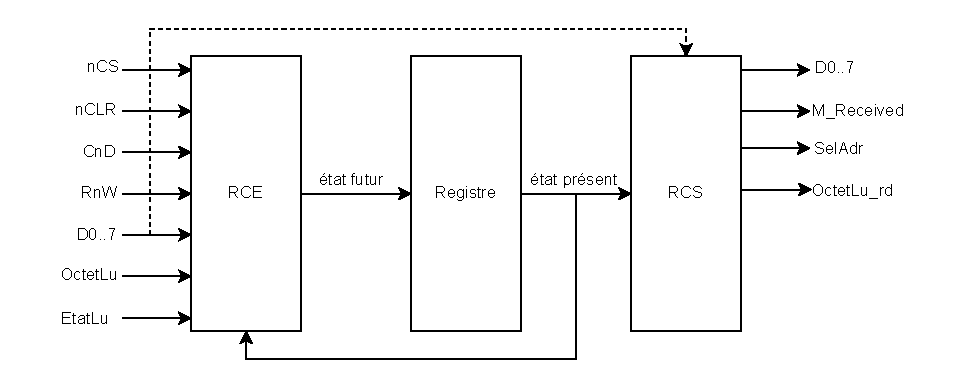
\includegraphics[width=0.8\linewidth]{images/inter/MEALY_Interface_Micro.pdf}
    \caption{Machine de Mealy – Interface microprocesseur}
    \label{fig:mealy_micro}
\end{figure}

\subsection{Architecture de la Mémoire FIFO}

La FIFO assure le stockage temporaire des octets reçus.  
Étant de complexité limitée, elle est décrite directement sous forme structurelle.

\begin{center}
\renewcommand{\arraystretch}{1.2}
\small
\begin{tabularx}{\textwidth}{|c||c|c|X|}
\hline
\textbf{Signal} & \textbf{Sens} & \textbf{Nature} & \textbf{Rôle fonctionnel} \\ \hline
DATA\_IN & Entrée & Données & Données reçues à stocker \\ 
WRITE & Entrée & Commande & Validation d’écriture \\ 
RESET & Entrée & Commande & Réinitialisation du contenu \\ 
DATA\_OUT & Sortie & Données & Données lues \\ 
READ & Entrée & Commande & Validation de lecture \\ 
\hline
\end{tabularx}
\end{center}

\begin{figure}[H]
    \centering
    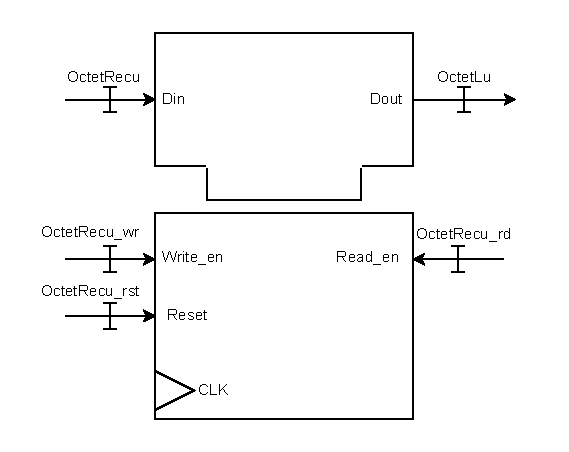
\includegraphics[width=0.8\linewidth]{images/inter/Implementation_FIFO.pdf}
    \caption{Implémentation structurelle de la mémoire FIFO}
    \label{fig:fifo}
\end{figure}

\subsection{Implémentation du Registre d’État}

Le registre d’état regroupe les informations relatives aux erreurs, au nombre d’octets reçus et à la validation des trames.

\begin{figure}[htbp]
    \centering
    \begin{subfigure}[b]{0.49\textwidth}
        \centering
        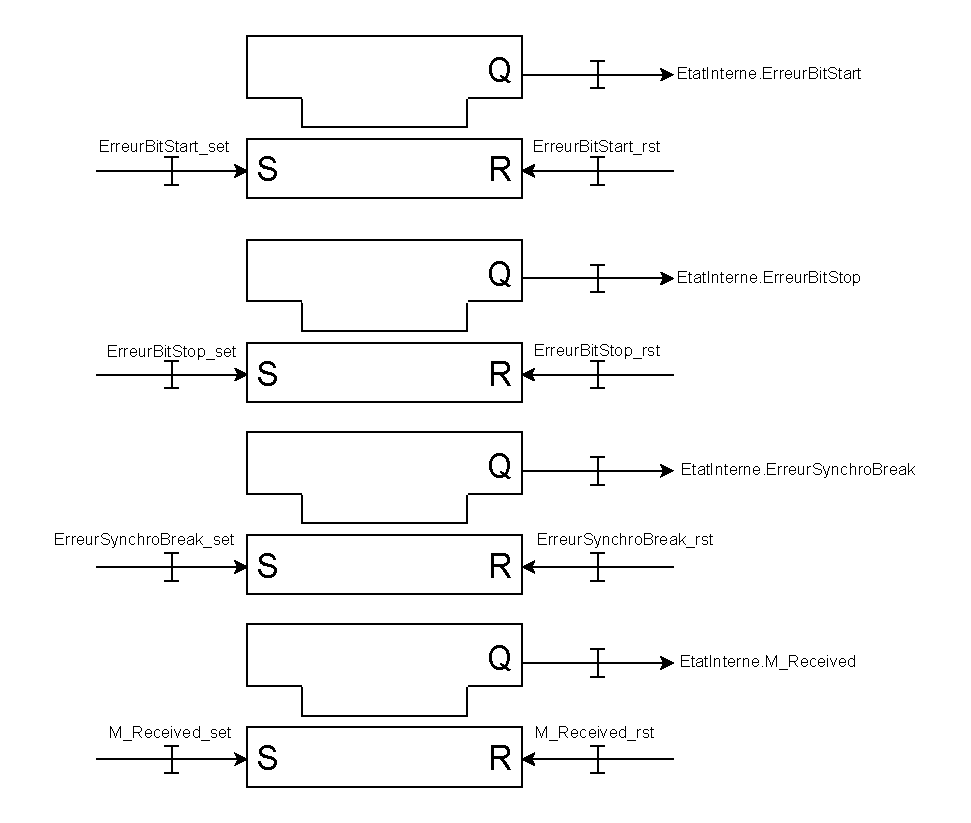
\includegraphics[width=\textwidth]{images/inter/Implementation_ETAT_Erreur.pdf}
        \caption{Mémorisation des erreurs détectées}
    \end{subfigure}
    \hfill
    \begin{subfigure}[b]{0.49\textwidth}
        \centering
        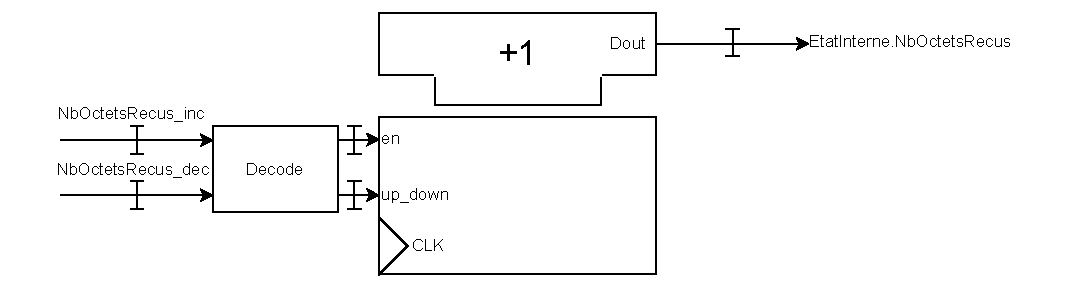
\includegraphics[width=\textwidth]{images/inter/Implementation_ETAT_NbOctets.pdf}
        \caption{Comptage des octets reçus}
    \end{subfigure}
    \caption{Implémentation structurelle du registre d’état au niveau RT}
    \label{fig:etat_impl}
\end{figure}


\section{Présentation du fonctionnement des fonctions}

\subsection{Interface MicroProcesseur}

Dans cette partie, nous avons initié une séance de travaux pratiques pour nous familiariser avec 
le logiciel HDL Designer. Le programme «Interface Microprocesseur», préalablement implémenté par 
les enseignants, respecte strictement les données présentées dans le TD et développées dans les 
sections précédentes du rapport. Nous allons l’étudier en détail afin de démontrer sa correspondance 
avec le modèle théorique.
\newline

Pour rappel, l’interface Microprocesseur a été conçue selon une machine séquentielle, tandis que 
la partie commande a été développée sur le modèle d’une machine de Mealy. Le code présenté respecte 
rigoureusement la structure des blocs : réseau combinatoire d’entrée, réseau combinatoire de sortie 
et registres correspondant à la machine à états.
\newline

\subsubsection{Synchronisation des Entrées}

\begin{lstlisting}[style=VHDLStyle, caption={Reseau Cominatoire d'entrée}]
InputProc_Synchro :  PROCESS(H, nRST)
BEGIN
  IF (nRST='0') THEN 
    nCS_Synchro <= '1';
    RnW_Synchro <= '1';
    CnD_Synchro <= '1';
    D07_Synchro <= (others => '0');
  ELSIF (H'EVENT AND H='1') THEN
    nCS_Synchro <= nCS;
    RnW_Synchro <= RnW;
    CnD_Synchro <= CnD;
    D07_Synchro <= D07;
  END IF;
END PROCESS InputProc_Synchro;
\end{lstlisting}

Ce bloc VHDL gère la synchronisation des signaux provenant du microprocesseur. Le processus \texttt{InputProc\_Synchro} lit les signaux d’entrée à chaque front montant de l’horloge \texttt{H} et les initialise lors de la mise à zéro \texttt{nRST}. Les signaux synchronisés (\texttt{nCS\_Synchro, RnW\_Synchro, CnD\_Synchro, D07\_Synchro}) sont ensuite utilisés par le reste de l’interface.

\subsubsection{Réseau Combinatoire de Sortie}

\begin{lstlisting}[style=VHDLStyle, caption={Reseau Cominatoire de Sortie}]
OutputProc_Comb : PROCESS(nCS_Synchro, CnD_Synchro, RnW_Synchro, EtatCourant, OctetLu, EtatLu)
BEGIN
  D07 <= (others => 'Z');
  OctetLu_RD <= '0';
  EtatLu_RST <= '0';
  DecNbOctet <= '0';
  CASE EtatCourant IS
    WHEN Attente =>
      IF (nCS_Synchro='0' AND CnD_Synchro='0' AND RnW_Synchro='1') THEN
        OctetLu_RD <= '1';
      END IF;
    WHEN LectureData =>
      D07 <= OctetLu;
      IF (nCS_Synchro='1') THEN
        DecNbOctet <= '1';
      END IF;
    WHEN LectureEtat =>
      D07 <= EtatLu;
      IF (nCS_Synchro='1') THEN
        EtatLu_RST <= '1';
      END IF;
    WHEN EcritureFiltre =>   
    END CASE;
END PROCESS OutputProc_Comb;
\end{lstlisting}

Le processus \texttt{OutputProc\_Comb} contrôle la sortie des données et des états vers le microprocesseur. Il met à jour les signaux \texttt{D07, OctetLu\_RD, EtatLu\_RST, DecNbOctet} en fonction de l’état courant de la machine et des signaux synchronisés d’entrée. La logique combinatoire assure la correspondance entre les actions de lecture/écriture et l’état de la machine.

\subsubsection{Réseau Combinatoire d'Entrée}

\begin{lstlisting}[style=VHDLStyle, caption={Registres}]
ClockedProc : PROCESS(H, nRST)
BEGIN
  IF (nRST='0') THEN
    EtatCourant <= Attente;
  ELSIF (H'EVENT AND H='1') THEN
    EtatCourant <= EtatSuivant;
  END IF;
END PROCESS ClockedProc;

NextStateProc : PROCESS(nCS_Synchro, CnD_Synchro, RnW_Synchro, EtatCourant)
BEGIN
  EtatSuivant <= EtatCourant;
  CASE EtatCourant IS
  WHEN Attente =>
    IF (nCS_Synchro='0' AND CnD_Synchro='0' AND RnW_Synchro='1') THEN
      EtatSuivant <= LectureData;
    ELSIF (nCS_Synchro='0' AND CnD_Synchro='1' AND RnW_Synchro='1') THEN
      EtatSuivant <= LectureEtat;
    ELSIF (nCS_Synchro='0' AND CnD_Synchro='0' AND RnW_Synchro='0') THEN
      EtatSuivant <= EcritureFiltre;
    ELSE
      EtatSuivant <= Attente;
    END IF;
    WHEN LectureData =>
      IF (nCS_Synchro='1') THEN
        EtatSuivant <= Attente;
      ELSE
        EtatSuivant <= LectureData;
      END IF;
    WHEN LectureEtat =>
      IF (nCS_Synchro='1') THEN
        EtatSuivant <= Attente;
      ELSE
        EtatSuivant <= LectureEtat;
      END IF;
    WHEN EcritureFiltre =>
      IF (nCS_Synchro='1') THEN
        EtatSuivant <= Attente;
      ELSE 
        EtatSuivant <= EcritureFiltre;
      END IF;
  END CASE;
END PROCESS NextStateProc;
\end{lstlisting}

Les processus \texttt{ClockedProc} et \texttt{NextStateProc} implémentent la machine séquentielle. \texttt{ClockedProc} met à jour l’état courant à chaque front montant de l’horloge et réinitialise l’état au démarrage. \texttt{NextStateProc} définit l’état suivant selon les conditions des signaux d’entrée et l’état courant, en suivant la logique de la machine de Mealy.

\subsubsection{Réseau Synchronisé de Sortie}

\begin{lstlisting}[style=VHDLStyle, caption={Reseau Synchronisé de Sortie}]
OutputProc_Synchro : PROCESS(H, nCLR)
BEGIN 
  IF (nCLR='0') THEN
    SelAdr <= (others => '0');
  ELSIF (H'EVENT AND H='1') THEN 
    CASE EtatCourant IS 
    WHEN EcritureFiltre =>
      IF (nCS_Synchro='1') THEN
        SelAdr <= D07_Synchro;
      END IF;
    WHEN OTHERS =>
    END CASE;
  END IF;
END PROCESS OutputProc_Synchro;
  
M_Received <= EtatLu(4);

\end{lstlisting}

Le processus \texttt{OutputProc\_Synchro} synchronise la sélection d’adresse \texttt{SelAdr} avec l’horloge \texttt{H}. Il est actif principalement pendant l’état \texttt{EcritureFiltre}, assurant que les données de l’entrée \texttt{D07\_Synchro} sont correctement mémorisées. Le signal \texttt{M\_Received} est également mis à jour pour refléter l’état du bit correspondant.

\subsection{Interface de Réception LIN}

L’interface de réception LIN a été étudiée sous la forme d’une machine séquentielle, composée d’une partie opérative et d’une partie commande.
La partie opérative est développée sous la forme d’un schéma fonctionnel comprenant différents blocs tels que des multiplexeurs et des compteurs/décompteurs.
La partie commande, quant à elle, a été modélisée sous la forme d’un automate, traduit en machine de Moore, puis implémenté en VHDL.

Voici un tableau recapitulant les entrées et les sorties du bloc Repetion LIN complet : 
\newline

\begin{center}
\renewcommand{\arraystretch}{1.2} % espace vertical
\small % pour uniformiser la taille du texte
    \begin{tabularx}{\textwidth}{|c||c|c|X|}
     \hline			
       \textbf{Signaux} & \textbf{Mode} & \textbf{Type} & \textbf{Description}  \\ \hline 
       LIN & IN & \texttt{STD\_LOGIC} & Bus de données d'entrée \\
       SelAdr & IN & \texttt{STD\_LOGIC\_VECTOR(7 DOWNTO 0)} & Sélection Adrress Composant \\
       OctetRecu & OUT & \texttt{STD\_LOGIC\_VECTOR(7 DOWNTO 0)} & Bus de données de sortie \\
       OctetRecu\_WR & OUT & \texttt{STD\_LOGIC} & Read / Write opération \\
       OctetRecu\_RST & OUT & \texttt{STD\_LOGIC} & Réinitialisation des données reçues \\
       Erreur\_Start & OUT & \texttt{STD\_LOGIC} & Bit d'erreur de Start \\
       Erreur\_Stop & OUT & \texttt{STD\_LOGIC} & Bit d'erreur de Stop\\
       Erreur\_SynchroBreak & OUT & \texttt{STD\_LOGIC} & Bit d'erreur de Synchro Break\\
       IncNbOctet & OUT & \texttt{STD\_LOGIC} & Flag de reception pour lecture \\
       MessageReceived\_SET & OUT & \texttt{STD\_LOGIC} & Indicateur de trame reçue \\
       NbOctetRecu\_RST & OUT & \texttt{STD\_LOGIC} & Réinitialisation du compteur d'octets \\
     \hline  
    \end{tabularx}
\end{center}

\subsubsection{Partie opérative}

La partie opérative, déjà définie dans la section Description de la solution architecturale, a été reprise sous forme de blocs fonctionnels.
Il a simplement été nécessaire de reproduire le schéma global dans HDL Designer, afin d’assurer la cohérence entre la conception théorique et la modélisation pratique.

Le schéma correspondant est présenté ci-dessous :

%%%%%%%%%%%%%%%%%%%%%%%%%%%%%%%%%%%%%%%%%%%%%%%%%%%%%%%%%%%%%%%%%%%%%%%%%%%%%%%%%%%%%%%%%%%%%%%%%
%\begin{figure}[H]
%    \centering
%    \includegraphics[width=0.95\linewidth]{images/presen/Schema_PO_RectionLin.png}
%    \caption{Schéma partie opérative réception LIN}
%    \label{fig:placeholder}
%\end{figure}
%%%%%%%%%%%%%%%%%%%%%%%%%%%%%%%%%%%%%%%%%%%%%%%%%%%%%%%%%%%%%%%%%%%%%%%%%%%%%%%%%%%%%%%%%%%%%%%%%

Voici aussi le tableau des entrées et sorties de la partie opérative : 

\begin{center}
\renewcommand{\arraystretch}{1.2} % espace vertical
\small % pour uniformiser la taille du texte
\begin{tabularx}{\textwidth}{|c||c|c|X|}
\hline			
\textbf{Signaux} & \textbf{Mode} & \textbf{Type} & \textbf{Description}  \\ 
\hline \hline

H & IN & \texttt{STD\_LOGIC} & Horloge principale du système. \\ 
Identifier & IN & \texttt{STD\_LOGIC\_VECTOR(7 DOWNTO 0)} & Identifiant du message reçu à comparer avec l’adresse sélectionnée. \\ 
LinSynchro & IN & \texttt{STD\_LOGIC} & Signal de synchronisation de trame LIN. \\ 
NbTbit\_0 & IN & \texttt{STD\_LOGIC} & Bit de configuration du nombre de bits de trame. \\ 
NbDataField\_0 & IN & \texttt{STD\_LOGIC} & Bit de configuration du nombre d’octets de données dans le champ Data. \\ 
SelAdr & IN & \texttt{STD\_LOGIC\_VECTOR(7 DOWNTO 0)} & Sélection de l’adresse du composant (comparée à Identifier). \\ 
nCLR & IN & \texttt{STD\_LOGIC} & Signal de réinitialisation asynchrone active à l’état bas. \\ 
n\_0 & IN & \texttt{STD\_LOGIC} & Signal de contrôle interne (sélection ou validation). \\ 
Error\_Start & OUT & \texttt{STD\_LOGIC} & Bit d’erreur sur le champ Start. \\ 
Error\_Stop & OUT & \texttt{STD\_LOGIC} & Bit d’erreur sur le champ Stop. \\ 
Error\_Synchro & OUT & \texttt{STD\_LOGIC} & Bit d’erreur de synchronisation (Synchro Break). \\ 
Identifieur\_en & OUT & \texttt{STD\_LOGIC} & Validation de l’identifiant reçu. \\ 
IncNbOctet & OUT & \texttt{STD\_LOGIC} & Incrémentation du compteur d’octets reçus. \\ 
MessageReceiveSet & OUT & \texttt{STD\_LOGIC} & Indique qu’une trame complète a été reçue. \\ 
NbDataField\_EN & OUT & \texttt{STD\_LOGIC} & Activation du champ de données (Data Field). \\ 
NbDataField\_load & OUT & \texttt{STD\_LOGIC} & Chargement du nombre d’octets de données. \\ 
NbOctetRecu\_RST & OUT & \texttt{STD\_LOGIC} & Réinitialisation du compteur d’octets reçus. \\ 
OctetRecu\_RST & OUT & \texttt{STD\_LOGIC} & Réinitialisation du registre d’octet reçu. \\ 
OctetRecu\_WR & OUT & \texttt{STD\_LOGIC} & Signal d’écriture de l’octet reçu. \\ 
OctetRecu\_en & OUT & \texttt{STD\_LOGIC} & Validation du registre d’octet reçu. \\ 
n\_Tbit\_Load & OUT & \texttt{STD\_LOGIC} & Chargement du registre associé au Tbit. \\ 
n\_Tbit\_en & OUT & \texttt{STD\_LOGIC} & Activation du registre Tbit. \\ 
n\_Tbit\_select & OUT & \texttt{STD\_LOGIC} & Sélection de la source ou mode du Tbit. \\ 
n\_en & OUT & \texttt{STD\_LOGIC} & Activation du signal ou compteur “n”. \\ 
n\_load & OUT & \texttt{STD\_LOGIC} & Chargement de la valeur “n”. \\ 
n\_select & OUT & \texttt{STD\_LOGIC} & Sélection de la source du signal “n”. \\ 
\hline

\end{tabularx}
\end{center}


\subsubsection{Partie Commande}

La partie commande consiste principalement à \textbf{traduire l’automate} présenté en figure~\ref{fig:automatereceptionlin} en \textbf{code VHDL}.  
Cette étape reste relativement simple, car elle repose sur la création de \textbf{trois processus principaux} :

\begin{enumerate}
    \item \textbf{Le réseau combinatoire d’entrée}, chargé de déterminer les \textit{états futurs} de l’automate en fonction des \textit{états présents} et des \textit{signaux d’entrée}.
    \item \textbf{Le réseau de registres}, synchronisé sur l’horloge, permettant de \textit{mémoriser les états} et d’assurer la transition entre les \textit{états présents} et les \textit{états futurs}.
    \item \textbf{Le réseau combinatoire de sortie}, qui met à jour les \textit{signaux de sortie} en fonction de l’état courant de l’automate.
\end{enumerate}

Voici le code suivant qui permet de traduire l'automate : 
\newline

\begin{lstlisting}[style=VHDLStyle, caption={Declaration des états}]
-- Etat de la machine
type CFM is (
    R_BRK_0, R_BRK_1,                -- Reception Break
    SYN_A, SYN_RST, SYN_RD, SYN_RSP, -- Synchro
    IDN_A, IDN_RST, IDN_RD, IDN_RSP, -- Identifier
    DAT_A, DAT_RST, DAT_RD, DAT_RSP, -- Datafield
    CHK_A, CHK_RST, CHK_RD, CHK_RSP, -- Checksum
    REPOS                            -- Repos
);
\end{lstlisting}

Dans une première étape, nous déclarons les différents états de l’automate sous la forme d’un type énuméré nommé \texttt{CFM}.
Chaque état correspond à une étape spécifique du processus de réception LIN, facilitant ainsi la gestion des transitions et des actions associées à chaque état.
\newline


\begin{lstlisting}[style=VHDLStyle, caption={Registres Reception Trame}]
-- Register
CFM_Register : process(H, nCLR)
begin
    if nCLR = '0' then
        P_CFM <= REPOS;
    elsif rising_edge(H) then
        P_CFM <= N_CFM;
    end if;
end process CFM_Register;
\end{lstlisting}

Dans ce code nous retrouvons la clock qui permet de synchroniser les états de l'automate avec le signal d'horloge H.
Le changement d'état se fait au front montant de l'horloge.
Le reset asynchrone nCLR permet de remettre l'automate dans son état initial
\newline

\begin{lstlisting}[style=VHDLStyle, caption={Réseau Combinatoire d’Entrée Reception Trame}]
-- Reseau Combinatoire d'Entree
CFM_RCE : process(P_CFM, H, Identifier, LinSynchro, NbTbit_0, NbDataField_0, SelAdr, nCLR, n_0)
begin
    -- Next State <= Present State
    N_CFM <= P_CFM;

    case P_CFM is
        when REPOS => -- Attente
            if LinSynchro = '0' then
                N_CFM <= R_BRK_0;
            end if;
        when R_BRK_0 => -- Synchro Break 0
            if NbTbit_0 = '1' AND LinSynchro = '1' then
                N_CFM <= R_BRK_1;
            elsif NbTbit_0 = '0' AND LinSynchro = '1' then
                N_CFM <= REPOS;
            elsif n_0 = '0' AND LinSynchro = '0' AND NbTbit_0 = '0' then
                N_CFM <= R_BRK_0;
            elsif NbTbit_0 = '0' AND LinSynchro = '0' AND n_0 = '1' then
                N_CFM <= R_BRK_0;
            end if;
        when R_BRK_1 => -- Synchro Break 1
            if n_0 = '1' AND LinSynchro = '1' then
                N_CFM <= SYN_A;
            elsif n_0 = '0' AND LinSynchro = '0' then
                N_CFM <= REPOS;
            elsif n_0 = '0' then
                N_CFM <= R_BRK_1;
            end if;
        when SYN_A => -- Attente bit Start Synchronisation
            if LinSynchro = '0' then
                N_CFM <= SYN_RST;
            end if;
        when SYN_RST => -- Reception Start Synchronisation
            if n_0 = '0' AND LinSynchro = '0' then
                N_CFM <= SYN_RD;
            elsif n_0 = '0' AND LinSynchro = '1' then
                N_CFM <= REPOS;
            elsif n_0 = '0' then
                N_CFM <= SYN_RST;
            end if;
        when SYN_RD => -- Reception Data Synchronisation
            if NbTbit_0 = '1' then
                N_CFM <= SYN_RSP;
            elsif n_0 = '1' AND NbTbit_0 = '0' then
                N_CFM <= SYN_RD;
            elsif n_0 = '0' then
                N_CFM <= SYN_RD;
            end if;
        when SYN_RSP => -- Reception bit Stop Synchronisation
            if n_0 = '1' AND LinSynchro = '1' then
                N_CFM <= IDN_A;
            elsif n_0 = '0' AND NbTbit_0 = '0' then
                N_CFM <= REPOS;
            elsif n_0 = '0' then
                N_CFM <= SYN_RSP;
            end if;
        when IDN_A => -- Attente bit Start Identifier
            if LinSynchro = '0' then
                N_CFM <= IDN_RST;
            end if;
        when IDN_RST => -- Reception bit Start Identifier
            if n_0 = '1' AND LinSynchro = '0' then
                N_CFM <= IDN_RD;
            elsif n_0 = '1' AND LinSynchro = '1' then
                N_CFM <= REPOS;
            elsif n_0 = '0' AND LinSynchro = '0' then
                N_CFM <= IDN_RST;
            end if;       
        when IDN_RD => -- Reception Data Identifier
            if NbTbit_0 = '1' AND n_0 = '1' then
                N_CFM <= IDN_RSP;
            elsif n_0 = '0' then
                N_CFM <= IDN_RD;
            elsif n_0 = '1' AND NbTbit_0 = '0' then
                N_CFM <= IDN_RD;
            end if;     
        when IDN_RSP => -- Reception bit Stop Identifier
            if n_0 = '1' AND LinSynchro = '1' then
                N_CFM <= DAT_A;
            elsif n_0 = '1' AND LinSynchro = '0' then
                N_CFM <= REPOS;
            elsif n_0 = '0' AND LinSynchro = '1' then
                N_CFM <= IDN_RSP;
            end if;   
        when DAT_A => -- Attente bit Start Datafield
            if LinSynchro = '0' then
                N_CFM <= DAT_RST;
            end if;   
        when DAT_RST => -- Reception bit Start Datafield
            if n_0 = '1' AND LinSynchro = '0' then
                N_CFM <= DAT_RD;
            elsif n_0 = '1' AND LinSynchro = '1' then
                N_CFM <= REPOS;
            elsif n_0 = '0' AND LinSynchro = '0' then
                N_CFM <= DAT_RST;
            end if;         
        when DAT_RD => -- Reception bit Data Datafield
            if NbTbit_0 = '1' AND LinSynchro = '1' then
                N_CFM <= DAT_RSP;
            elsif n_0 = '1' AND NbTbit_0 = '0' then
                N_CFM <= DAT_RD;
            elsif n_0 = '0' then
                N_CFM <= DAT_RD;
            end if;          
        when DAT_RSP => -- Reception bit Stop Datafield
		        if n_0 = '0' AND NbDataField_0 = '1' AND LinSynchro = '1' then
                N_CFM <= CHK_A;
            elsif NbDataField_0 = '0' AND n_0 = '1'AND LinSynchro = '1' then
                N_CFM <= DAT_A;
            elsif n_0 = '1' AND LinSynchro = '0' then
                N_CFM <= REPOS;
            elsif n_0 = '0' AND LinSynchro = '1'then
                N_CFM <= DAT_RSP;
            end if;   
        when CHK_A => -- Attente bit Start Checksum
            if LinSynchro = '0' then
                N_CFM <= CHK_RST;
            end if;           
        when CHK_RST => -- Reception bit Start Checksum
            if n_0 = '1' AND LinSynchro = '0' then
                N_CFM <= CHK_RD;
            elsif n_0 = '1' AND LinSynchro = '1' then
                N_CFM <= REPOS;
			elsif n_0 = '0' AND LinSynchro = '0' then
                N_CFM <= CHK_RST;
            end if;         
        when CHK_RD => -- Reception bit Data Checksum
            if NbTbit_0 = '1' AND LinSynchro = '1' then
                N_CFM <= CHK_RSP;
            elsif n_0 = '1' AND NbTbit_0 = '0' then
                N_CFM <= CHK_RD;
            elsif n_0 = '0' then
                N_CFM <= CHK_RD;
            end if;          
        when CHK_RSP => -- Reception bit Stop Checksum
            if n_0 = '1' AND LinSynchro = '1' AND Identifier = SelAdr then
                N_CFM <= REPOS; -- Fin de Trame Complete
            elsif n_0 = '1' AND LinSynchro = '1' AND Identifier /= SelAdr then
                N_CFM <= REPOS;
            elsif n_0 = '0' AND LinSynchro = '0' then
                N_CFM <= REPOS;
            elsif n_0 = '0' AND LinSynchro = '1' then
                N_CFM <= CHK_RSP;
            end if;               
    end case;
    
end process CFM_RCE;
\end{lstlisting}

Ce code VHDL traduit l’automate de réception LIN en utilisant un processus combinatoire nommé \texttt{CFM\_RCE}.
Il détermine l’état suivant (\texttt{N\_CFM}) en fonction de l’état actuel (\texttt{P\_CFM}) et des signaux d’entrée tels que \texttt{LinSynchro}, \texttt{NbTbit\_0}, \texttt{Identifier}, etc.
Chaque état de l’automate est représenté par une branche dans la structure \texttt{CASE}, avec des conditions spécifiques pour les transitions entre états.
\newline

\begin{lstlisting}[style=VHDLStyle, caption={Réseau Combinatoire de Sortie Reception Trame}]
  -- Reseau Combinatoire de Sortie
CFM_RES : process(P_CFM, H, Identifier, LinSynchro, NbTbit_0, NbDataField_0, SelAdr, nCLR, n_0 )
begin
  -- Valeurs par defaut
  Error_Start       <= '0';
  Error_Stop        <= '0';
  Error_Synchro     <= '0';
  Identifieur_en    <= '0';
  IncNbOctet        <= '0';
  MessageReceiveSet <= '0';
  NbDataField_EN    <= '0';
  NbDataField_load  <= '0';
  NbOcyeyRecu_RST   <= '0';
  OctetRecu_RST     <= '0';
  OctetRecu_WR      <= '0';
  OctetRecu_en      <= '0';
  n_Tbit_Load       <= '0';
  n_Tbit_en         <= '0';
  n_Tbit_select     <= '0';
  n_en              <= '0';
  n_load            <= '0';
  n_select          <= '0';

  case P_CFM is 
    when REPOS => -- Attente
      if LinSynchro = '0' then 
        n_select       <= '0';
        n_load         <= '1';
        n_en           <= '1';
        n_Tbit_select  <= '0';
        n_Tbit_en      <= '1';
        n_Tbit_Load    <= '1';
      end if;

    when R_BRK_0 => -- Synchro Break 0
      if NbTbit_0 = '1' and LinSynchro = '1' then
        n_select <= '0';
        n_en     <= '1';
        n_load   <= '1';
      elsif NbTbit_0 = '0' and LinSynchro = '1' then
        Error_Synchro <= '1';
      elsif NbTbit_0 = '0' and LinSynchro = '0' and n_0 = '1' then
        n_Tbit_en <= '1';
        n_select  <= '0';
        n_load    <= '1';
        n_en      <= '1';
      elsif n_0 = '0' AND LinSynchro = '0' AND NbTbit_0 = '0' then 
         n_en <= '1';
      end if;

    when R_BRK_1 => -- Synchro Break 1 
      if n_0 = '1' and LinSynchro = '0' then
        -- Nothing
      elsif n_0 = '0' and LinSynchro = '0' then
        Error_Synchro <= '1';
      elsif n_0 = '0' then
        n_en <= '1';
      end if;
      
    when SYN_A => -- Attente bit Start Synchronisation
        if LinSynchro = '0' then
            n_select  <= '0';
            n_load    <= '1';
            n_en      <= '1';
        end if;
        
    when SYN_RST => -- Reception Start Synchronisation
        if n_0 = '0' AND LinSynchro = '0' then
            n_select       <= '1'; -- passage de fin de front a milieu bit
            n_load         <= '1';
            n_en           <= '1';
            n_Tbit_select  <= '1';
            n_Tbit_en      <= '1';
            n_Tbit_Load    <= '1';
        elsif n_0 = '0' AND LinSynchro = '1' then
            Error_Start    <= '1';
        elsif n_0 = '0' then
            n_en           <= '1';
        end if;
        
    when SYN_RD => -- Reception Data Synchronisation
        if NbTbit_0 = '1' then
            n_select       <= '0';
            n_load         <= '1';
            n_en           <= '1';
        elsif n_0 = '1' AND NbTbit_0 = '0' then
            n_select       <= '0';
            n_load         <= '1';
            n_en           <= '1';
            n_Tbit_en      <= '1';
            OctetRecu_en   <= '1';
        elsif n_0 = '0' then
            n_en           <= '1';
        end if;
        
    when SYN_RSP => -- Reception bit Stop Synchronisation
        if n_0 = '1' AND LinSynchro = '1' then
            OctetRecu_WR   <= '1';
            n_select       <= '1';
            n_load         <= '1';
            n_en           <= '1';
        elsif n_0 = '0' AND NbTbit_0 = '0' then
            Error_Stop     <= '1';
        elsif n_0 = '0' then
            n_en           <= '1';
        end if;
        
    when IDN_A => -- Attente bit Start Identifier
        if LinSynchro = '0' then
            n_select       <= '0';
            n_load         <= '1';
            n_en           <= '1';
        end if;
        
    when IDN_RST => -- Reception bit Start Identifier
        if n_0 = '1' AND LinSynchro = '0' then
            n_select       <= '0';
            n_load         <= '1';
            n_en           <= '1';
            n_Tbit_select  <= '1';
            n_Tbit_Load    <= '1';
            n_Tbit_en      <= '1';
        elsif n_0 = '1' AND LinSynchro = '1' then
            Error_Start    <= '1';
        elsif n_0 = '0' AND LinSynchro = '0' then
            n_en           <= '1';
        end if;   
            
    when IDN_RD => -- Reception Data Identifier
        if NbTbit_0 = '1' AND n_0 = '1' then
            n_select       <= '0';
            n_load         <= '1';
            n_en           <= '1';
			OctetRecu_en   <= '1';
        elsif n_0 = '0' then
            n_en           <= '1';
        elsif n_0 = '1' AND NbTbit_0 = '0' then
			n_select       <= '0';
			n_load         <= '1';
            n_en           <= '1';
			n_Tbit_en      <= '1';
            OctetRecu_en   <= '1';
        end if; 
            
    when IDN_RSP => -- Reception bit Stop Identifier
        if n_0 = '1' AND LinSynchro = '1' then
            OctetRecu_en   <= '1';
			      NbDataField_EN <= '1';
			      Identifieur_en <= '1';
			      NbDataField_load <= '1';
        elsif n_0 = '0' AND LinSynchro = '0' then
            Error_Stop     <= '1';
        elsif n_0 = '0' AND LinSynchro = '1' then
            n_select       <= '0';
            n_load         <= '0';
            n_en           <= '1';
        end if;   
        
    when DAT_A => -- Attente bit Start Datafield
        if LinSynchro = '0' then
            n_select       <= '0';
            n_load         <= '1';
            n_en           <= '1';
        end if;   
        
    when DAT_RST => -- Reception bit Start Datafield
        if n_0 = '1' AND LinSynchro = '0' then
            n_select       <= '0';
            n_load         <= '1';
            n_en           <= '1';
            n_Tbit_select  <= '1';
            n_Tbit_Load    <= '1';
            n_Tbit_en      <= '1';
        elsif n_0 = '1' AND LinSynchro = '1' then
            Error_Start    <= '1';
        elsif n_0 = '0' AND LinSynchro = '0' then
            n_en           <= '1';
        end if;  
               
    when DAT_RD => -- Reception bit Data Datafield
        if NbTbit_0 = '1' AND LinSynchro = '1' then
            n_select       <= '0';
            n_load         <= '1';
            n_en           <= '1';
            OctetRecu_en   <= '1';
        elsif n_0 = '0' then
            n_en           <= '1';
        elsif n_0 = '1' AND NbTbit_0 = '0' then
            n_select       <= '0';
            n_load         <= '1';
            n_en           <= '1';
            n_Tbit_en      <= '1';
            OctetRecu_en   <= '1';
        end if; 
                 
   	when DAT_RSP => -- Reception bit Stop Datafield
		    if n_0 = '0' AND NbDataField_0 = '1' AND LinSynchro = '1' then
    			   OctetRecu_WR   <= '1';
    			   n_select       <= '0';
    			   n_load         <= '1';
    			   n_en           <= '1';
    			   IncNbOctet     <= '1';
    		  elsif NbDataField_0 = '0' AND n_0 = '1'AND LinSynchro = '1' then
    			   OctetRecu_WR   <= '1';
    			   NbDataField_EN <= '1';
    			   n_select       <= '0';
    			   n_load         <= '1';
    			   n_en           <= '1';
    			   IncNbOctet     <= '1';
    		  elsif n_0 = '1' AND LinSynchro = '0' then
    		    Error_Stop     <= '1';
 		    elsif n_0 = '0' AND LinSynchro = '1'then
    			   n_en           <= '1';
    		end if;  
          
    when CHK_A => -- Attente bit Start Checksum
        if LinSynchro = '0' then
            n_select       <= '0';
            n_load         <= '1';
            n_en           <= '1';
        end if;   
                
    when CHK_RST => -- Reception bit Start Checksum
    		if n_0 = '1' AND LinSynchro = '0' then
                n_select       <= '0';
                n_load         <= '1';
                n_en           <= '1';
                n_Tbit_select  <= '1';
    		elsif n_0 = '1' AND LinSynchro = '1' then
                Error_Start    <= '1';
    		elsif n_0 = '0' AND LinSynchro = '0' then
                n_en           <= '1';
      end if;  
               
    when CHK_RD => -- Reception bit Data Checksum
    		if NbTbit_0 = '1' AND LinSynchro = '1' then
                n_select       <= '0';
                n_load         <= '1';
                n_en           <= '1';
    		elsif n_0 = '1' AND NbTbit_0 = '0' then
                n_en           <= '1';
    		elsif n_0 = '0' then
                n_Tbit_en      <= '1';
                n_select       <= '0';
                n_load         <= '1';
                n_en           <= '1';
                OctetRecu_en   <= '1';
                Identifieur_en    <= '1';
                NbDataField_load  <= '1';
                NbDataField_EN    <= '1';
      end if;  
                
    when CHK_RSP => -- Reception bit Stop Checksum
        if n_0 = '0' AND LinSynchro = '1' AND Identifier = SelAdr then
            MessageReceiveSet <= '1';
            NbOcyeyRecu_RST   <= '1';
        elsif n_0 = '0' AND LinSynchro = '1' AND Identifier /= SelAdr then
            MessageReceiveSet <= '1';
            NbOcyeyRecu_RST   <= '1';
        elsif n_0 = '0' AND LinSynchro = '0' then
            Error_Stop     <= '1';
        elsif n_0 = '0' then
            n_en           <= '1';
        end if;                         
        
    when others =>
      -- Sec 
      null;
  end case;
end process CFM_RES;
\end{lstlisting}

Ce code VHDL implémente le réseau combinatoire de sortie (\texttt{CFM\_RES}) pour l’automate de réception LIN.
Il met à jour les signaux de sortie tels que \texttt{Error\_Start}, \texttt{Error\_Stop}, \texttt{OctetRecu\_WR}, etc., en fonction de l’état actuel (\texttt{P\_CFM}) et des signaux d’entrée.
Chaque état de l’automate est géré dans une structure \texttt{CASE}, avec des conditions spécifiques pour définir les actions à entreprendre dans chaque état.
Des valeurs par défaut sont également définies au début du processus pour éviter des comportements indésirlés.  
\newline

Une fois ces processus implémentés, il nous reste qu'a les assemblés pour ne formé qu'une machine Complete.
\newline

%%%%%%%%%%%%%%%%%%%%%%%%%%%%%%%%%%%%%%%%%%%%%%%%%%%%%%%%%%%%%%%%%%%%%%%%%%%%%%%%%%%%%%%%%%%%%%%%%
%\begin{figure}[H]
%    \centering
%    \includegraphics[width=0.95\linewidth]{images/presen/Schema_complet_RectionLin.png}
%    \caption{Machine Séquentielle réception LIN}
%    \label{fig:placeholder}
%\end{figure}
%%%%%%%%%%%%%%%%%%%%%%%%%%%%%%%%%%%%%%%%%%%%%%%%%%%%%%%%%%%%%%%%%%%%%%%%%%%%%%%%%%%%%%%%%%%%%%%%%

Le schéma complet de l’interface de réception LIN est présenté ci-dessus, illustrant l’intégration des différentes parties opératives et commandes ( Répresentant la machine séquentielle ).
\newline

\subsection{FIFO}

La mémoire FIFO (First In, First Out) a été conçue pour stocker temporairement les données reçues via l’interface LIN avant leur traitement ultérieur.
Elle est structurée autour d'un composant clef, la FIFO.
Cette section à été réaliser sur un schéma blocs, en reprenant les concepts vus en cours.
\newline

%%%%%%%%%%%%%%%%%%%%%%%%%%%%%%%%%%%%%%%%%%%%%%%%%%%%%%%%%%%%%%%%%%%%%%%%%%%%%%%%%%%%%%%%%%%%%%%%%
%\begin{figure}[H]
%    \centering
%    \includegraphics[width=0.95\linewidth]{images/presen/Schema_FIFO.png}
%    \caption{Schéma bloc FIFO}
%    \label{fig:placeholder}
%\end{figure}
%%%%%%%%%%%%%%%%%%%%%%%%%%%%%%%%%%%%%%%%%%%%%%%%%%%%%%%%%%%%%%%%%%%%%%%%%%%%%%%%%%%%%%%%%%%%%%%%%

\subsection{Etat Interne}

Etat interne est un composant VHDL qui gère les états internes du système de réception LIN. 
Le systeme à été conçu pour suivre et contrôler les différentes étapes du processus de réception des trames LIN.
L'Objectifs étant d'additionner des fonctionnalités de contrôle et de gestion des états internes pour ne formé qu'une seul trame.
\newline

Ce systeme à lui aussi été conçu sous la forme d'un schéma bloc, reprenant les concepts vus en cours. Avec des bascules D, des compteurs et l'ajout de OR pour gérer les RESET.
\newline

%%%%%%%%%%%%%%%%%%%%%%%%%%%%%%%%%%%%%%%%%%%%%%%%%%%%%%%%%%%%%%%%%%%%%%%%%%%%%%%%%%%%%%%%%%%%%%%%%
%\begin{figure}[H]
%    \centering
%    \includegraphics[width=0.95\linewidth]{images/presen/Schema_ETATINTERNE.png}
%    \caption{Schéma bloc FIFO}
%    \label{fig:placeholder}
%\end{figure}
%%%%%%%%%%%%%%%%%%%%%%%%%%%%%%%%%%%%%%%%%%%%%%%%%%%%%%%%%%%%%%%%%%%%%%%%%%%%%%%%%%%%%%%%%%%%%%%%%


\section{Simulation des fonctions}

\subsection{Interface Microprocesseur}

Dans cette section, nous présentons la simulation du bloc \textit{Interface Microprocesseur} et l’analyse des chronogrammes obtenus.  
La simulation a été réalisée à l’aide d’un \textit{testbench}, implémenté sous la forme d’un bloc nommé \texttt{EnvTest\_InterfaceMicroprocesseur}, connecté au composant \texttt{InterfaceMicroprocesseur}.  
L’objectif est de vérifier la conformité du fonctionnement par rapport à l’automate décrit dans la section \textit{Architecture}.

\begin{figure}[H]
    \centering
    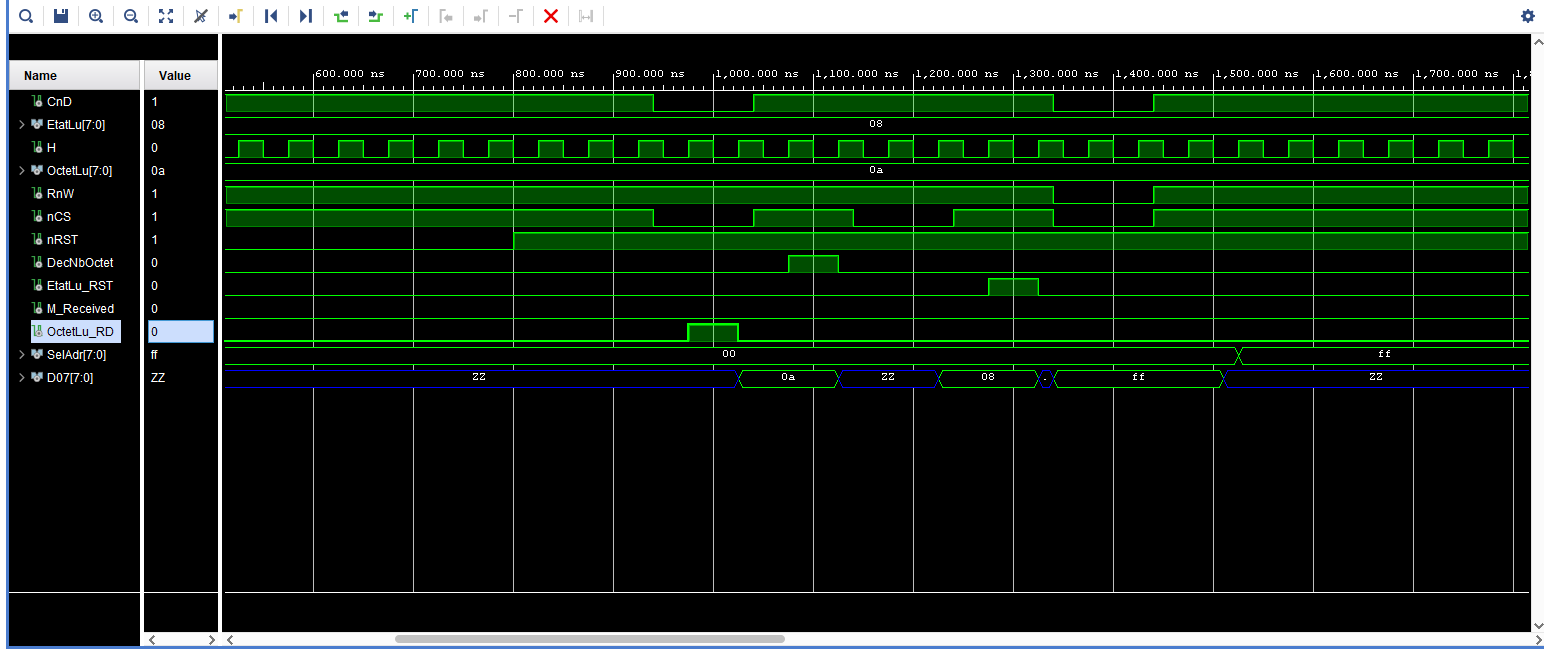
\includegraphics[width=0.95\linewidth]{images//Simulation/Chrono.png}
    \caption{Chronogramme de simulation de l’Interface Microprocesseur}
    \label{fig:placeholder}
\end{figure}

Le testbench (fourni en annexe) a pour rôle de reproduire l’environnement dans lequel le composant est amené à fonctionner.  
Il émule le comportement d’un microprocesseur en générant automatiquement les stimuli nécessaires à la validation du bloc testé.

\subsubsection{Déclarations et signaux}
Le testbench commence par la déclaration des librairies \texttt{IEEE}, nécessaires à la manipulation des types logiques et des vecteurs binaires.  
Les principaux signaux utilisés sont :
\begin{itemize}
  \item \texttt{CnD}, \texttt{RnW}, \texttt{nCS}, \texttt{nRST}, \texttt{H} : lignes de contrôle classiques d’une interface microprocesseur (commande/données, lecture/écriture, sélection du composant, reset, horloge),
  \item \texttt{OctetLu}, \texttt{EtatLu}, \texttt{SelAdr}, \texttt{D07} : bus de données et d’adresses sur 8 bits,
  \item \texttt{DecNbOctet}, \texttt{EtatLu\_RST}, \texttt{M\_Received}, \texttt{OctetLu\_RD} : signaux internes utilisés pour la communication avec le composant testé.
\end{itemize}

\subsubsection{Instanciation du composant testé}
Le composant \texttt{InterfaceMicroprocesseur} est instancié dans l’architecture de simulation.  
Il est relié à l’ensemble des signaux déclarés, permettant ainsi l’observation de son comportement face aux stimuli générés.

\subsubsection{Environnement de test}
Le composant \texttt{EnvTest\_InterfaceMicroprocesseur} simule le rôle du microprocesseur en générant automatiquement les signaux nécessaires :
\begin{itemize}
  \item génération de l’horloge (\texttt{H}),
  \item gestion du reset global (\texttt{nRST}),
  \item activation des commandes de lecture/écriture (\texttt{RnW}, \texttt{CnD}, \texttt{nCS}),
  \item pilotage du bus de données (\texttt{D07}).
\end{itemize}

Cet environnement est donné par plusieurs paramètres génériques :
\begin{itemize}
  \item \texttt{CLOCK\_PERIOD} : période d’horloge (50 ns),
  \item \texttt{RESET\_OFFSET} et \texttt{RESET\_DURATION} : moment et durée du reset (500 ns et 300 ns),
  \item \texttt{ACCESS\_TIME} et \texttt{HOLD\_TIME} : contraintes temporelles d’accès et de maintien (40 ns et 70 ns).
\end{itemize}

\begin{figure}[H]
    \centering
    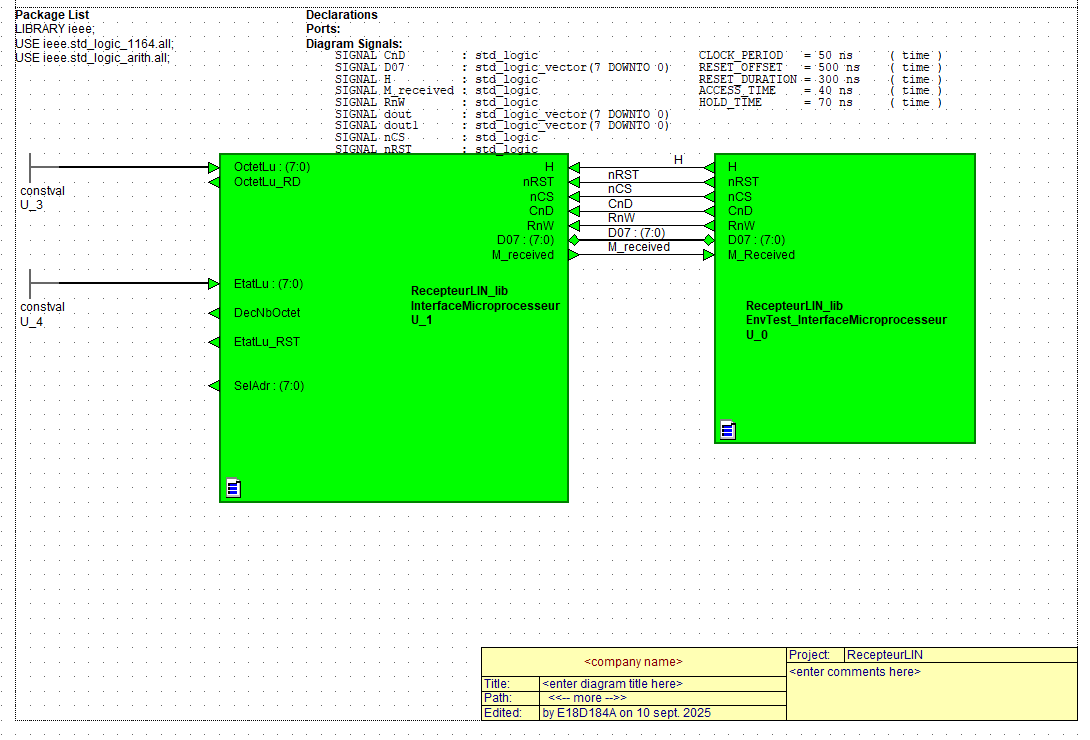
\includegraphics[width=0.95\linewidth]{images/Simulation/banc_test.png}
    \caption{Block Diagramme de test de l’Interface Microprocesseur}
    \label{fig:placeholder}
\end{figure}

\subsubsection{Stimuli supplémentaires}
Un processus spécifique (\texttt{StimProc}) complète la génération des signaux.  
Après la fin du reset, il impose des valeurs constantes sur certaines lignes :
\begin{itemize}
  \item \texttt{OctetLu} $\leftarrow$ 10 (codé sur 8 bits),
  \item \texttt{EtatLu} $\leftarrow$ 8 (codé sur 8 bits).
\end{itemize}
Ces valeurs permettent de vérifier la gestion correcte des données reçues par l’interface.  
La simulation est ensuite maintenue en attente infinie.

\subsubsection{Analyse du chronogramme de simulation}
L’analyse du chronogramme met en évidence le comportement attendu du composant :
\begin{itemize}
  \item lorsque les signaux de contrôle actifs à l’état bas (\texttt{nRST}, \texttt{nCS}) sont à l’état haut, aucune action n’est effectuée,
  \item lorsque ces signaux sont activés (passage à l’état bas), le composant réagit conformément à l’automate interne,
  \item les signaux \texttt{RnW} et \texttt{CnD} permettent de sélectionner respectivement les opérations de lecture/écriture et le type d’accès (commande ou données),
  \item les valeurs imposées sur \texttt{OctetLu} et \texttt{EtatLu} sont correctement lues via le bus de données \texttt{D07}.
\end{itemize}

Ce chronogramme confirme ainsi le bon fonctionnement du composant \texttt{InterfaceMicroprocesseur} :  
après la levée du reset, l’environnement de test génère des cycles de lecture et d’écriture auxquels le composant répond correctement, en échangeant les données prévues et en activant les signaux de contrôle appropriés.


\section{Synthèse des fonctions}

Une fois la validation en simulation des différents blocs effectuée, il est nécessaire de réaliser la synthèse sur FPGA afin d’observer les ressources logiques attribuées à notre système. 
Dans le cadre de ce projet, nous avons utilisé un FPGA \textit{AMD Xilinx Artix-7}, plus précisément le modèle \texttt{7A35TCPG236}. 
L’objectif de cette étape est d’analyser les ressources logiques mobilisées, ainsi que les éléments matériels effectivement utilisés par notre conception.
\newline

\subsection{Interface Microprocesseur}

Le schéma RTL (\textit{Register Transfer Level}) représente une implémentation 
synthétisée d’un module matériel décrit en VHDL ou Verilog. 
Il illustre les registres, les multiplexeurs, les portes logiques, 
ainsi que la logique séquentielle et combinatoire du circuit.


\begin{figure}[H]
    \centering
    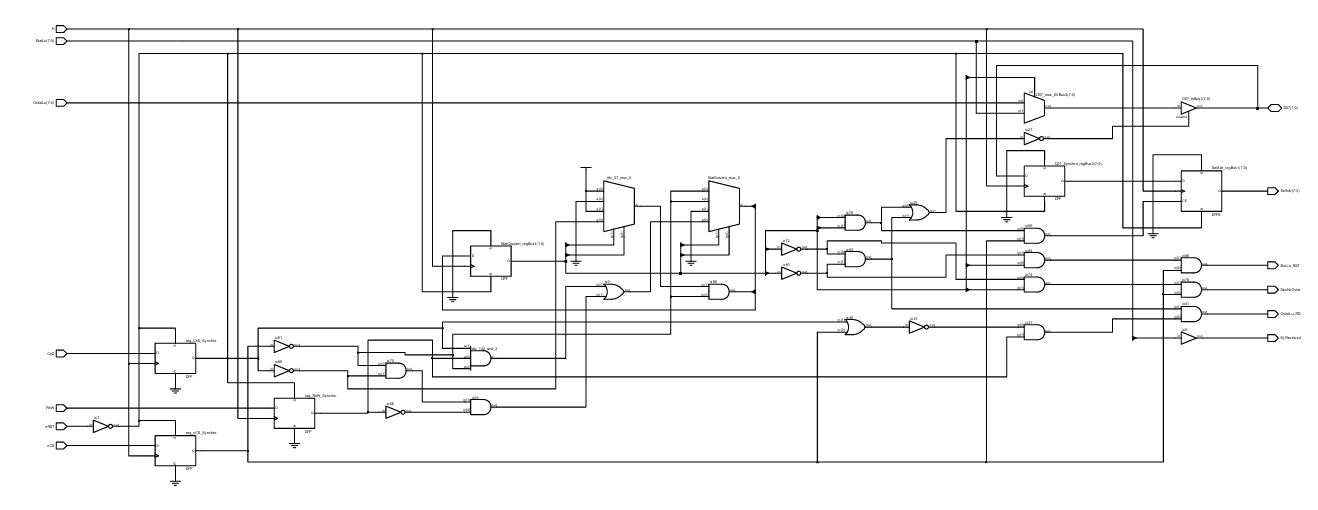
\includegraphics[width=0.9\linewidth]{images/Synthe/RTL_Shematic.png}
    \caption{Schéma RTL InterfaceMicroprocesseur}
    \label{fig:placeholder}
\end{figure}

\subsection*{Structure générale}
Le schéma peut être décomposé en plusieurs parties :
\begin{itemize}
    \item \textbf{Entrées principales} : signaux tels que 
    \texttt{H}, \texttt{CnD}, \texttt{RnW}, \texttt{nRST}, \texttt{nCS}, etc.
    \item \textbf{Registres (Flip-Flops D)} : éléments synchronisés par l’horloge, 
    servant à mémoriser l’état interne du circuit.
    \item \textbf{Multiplexeurs (MUX)} : permettent de sélectionner une donnée 
    parmi plusieurs, selon les conditions de contrôle.
    \item \textbf{Logique combinatoire} : réalisée par des portes AND, OR, NOT 
    et XOR, afin de générer les conditions de transition et les sorties.
    \item \textbf{Sorties} : plusieurs signaux dérivés de l’état interne, 
    comme \texttt{State\_XX}, \texttt{Output\_XX}, etc.
\end{itemize}

\subsection*{Fonctionnement global}
Le circuit implémente une \textbf{machine à états finis} :
\begin{itemize}
    \item Les \textbf{registres} contiennent l’état courant.
    \item La \textbf{logique combinatoire} calcule l’état suivant 
    en fonction de l’état courant et des entrées.
    \item Les \textbf{multiplexeurs} dirigent les transitions entre états.
    \item Les \textbf{sorties} sont activées ou désactivées selon l’état courant 
    et certaines combinaisons d’entrées.
\end{itemize}

\begin{figure}[H]
    \centering
    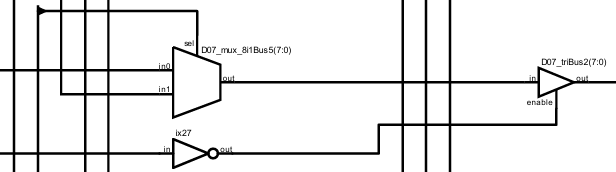
\includegraphics[width=0.9\linewidth]{images/Synthe/mux_tris.png}
    \caption{Partie opérative avec multiplexeur et Tristate : InterfaceMicroprocesseur}
    \label{fig:placeholder}
\end{figure}

De plus, nous pouvons retrouver la partie opérative dessinée en classe, lors de nos TD, qui permet, 
grâce à un multiplexeur, de sélectionner \textbf{EtalLu} ou \textbf{OctetLu} pour l'envoyer vers 
une porte \textbf{Tristate}.  
Cela démontre la cohérence entre la réalisation théorique et la mise en œuvre pratique.
\newline

À la suite de la synthèse logique nous pouvons avoir la la synthèse matériel qui transforme la 
logique en ressource matérielle.

\begin{figure}[H]
    \centering
    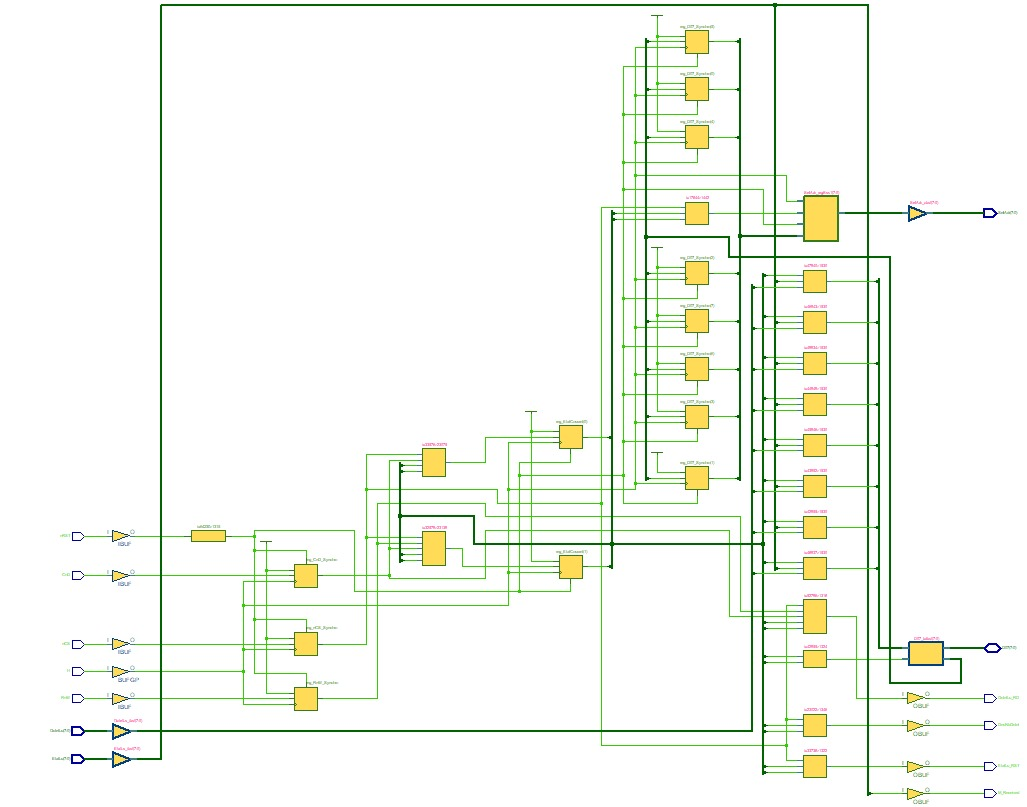
\includegraphics[width=0.9\linewidth]{images/Synthe/RTL_HARD_HDL.jpg}
    \caption{Synthese matérielle InterfaceMicroprocesseur}
    \label{fig:placeholder}
\end{figure}

Cette transformation consiste à mapper les éléments logiques du schéma RTL, tels que les portes 
\textbf{ AND, OR, NOT} ou les \textbf{multiplexeurs}, sur les \textbf{ressources matérielles 
physiques} disponibles dans le FPGA, notamment :  
\newline

\begin{itemize}
    \item \textbf{LUT (Look-Up Tables)} : les fonctions combinatoires, comme les portes logiques ou les multiplexeurs, sont réalisées à l’aide de LUT. Chaque LUT peut implémenter n’importe quelle fonction booléenne sur un nombre limité d’entrées, ce qui permet de reproduire fidèlement la logique définie dans le HDL.
    \item \textbf{Flip-flops} : les éléments séquentiels tels que les registres ou les bascules sont mappés sur des flip-flops pour stocker les bits et synchroniser les signaux dans le temps.
    \item \textbf{Buffers} : certains chemins logiques nécessitent des buffers pour renforcer les signaux ou adapter les niveaux électriques, garantissant ainsi la stabilité et l’intégrité du routage sur la puce.
\end{itemize}

Grâce à cette conversion, le design passe d’une \textbf{représentation abstraite de la logique} à une \textbf{implémentation matérielle concrète}, optimisée pour le FPGA cible. Cela permet non seulement de visualiser l’organisation physique des composants.
\newline

\section{Routages des Fonctions
}
\subsection{Interface Microprocesseur}

Après l'étape de \textbf{synthèse}, nous pouvons nous intéresser à l'assignation des ressources 
matérielles du système.\\
Pour cela, nous utilisons le logiciel \textbf{Vivado} (étant donné que les outils de HDL n'étaient 
pas disponibles le jour du TP), qui permet de générer un schéma RTL ainsi qu'une vue du routage 
associé à l'interface microprocesseur.
\newline

Dans un premier temps, Nous allons resynthétiser le design afin d'obtenir le schéma RTL.
Ce schéma, présenté ci-dessous, illustre les ressources logiques utilisées pour implémenter 
l'interface microprocesseur.
\newline

\resizebox{\textwidth}{!}{%
    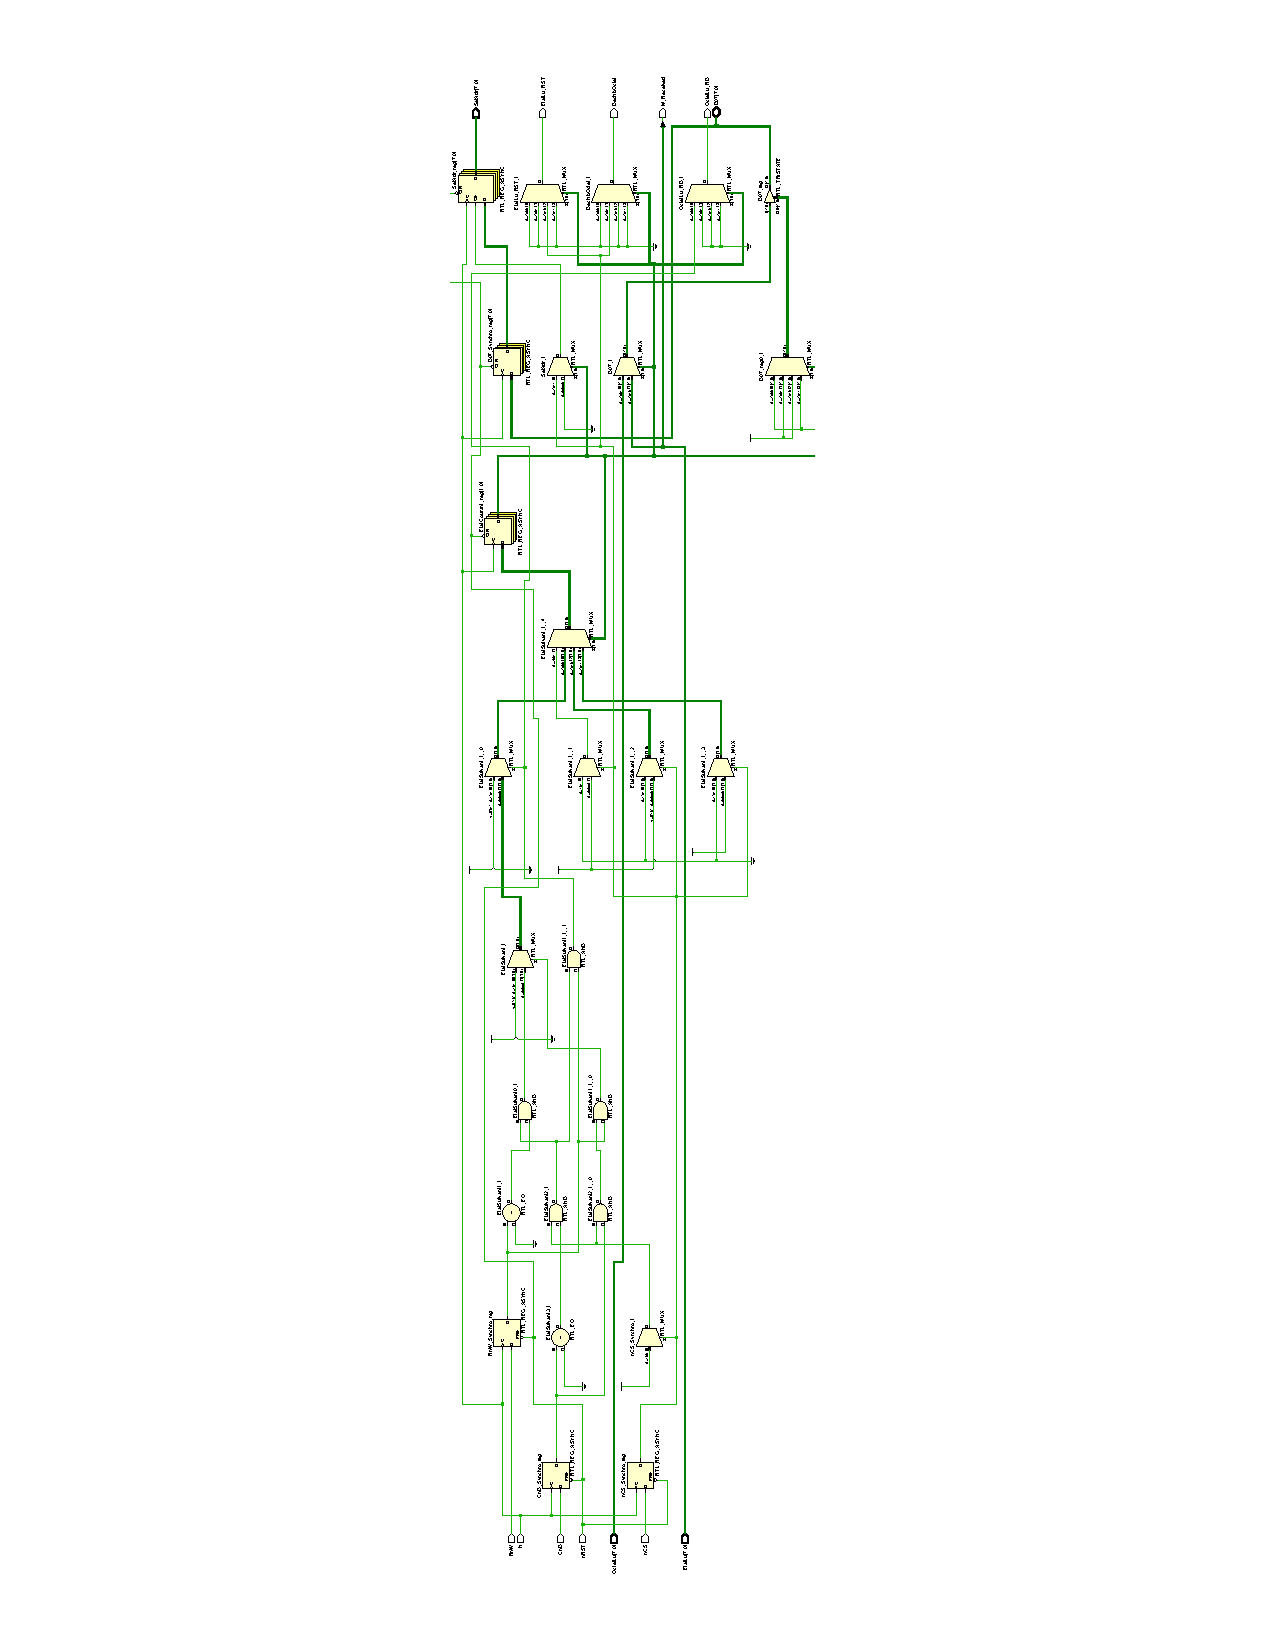
\includegraphics[angle=-90]{images/Routage/pdf_recadre_recadre.pdf}%
}

\vspace{10pt}

Par la suite, nous pouvons également observer la synthèse matérielle réalisée sur Vivado, qui 
transforme les ressources logiques en ressources matérielles pour le FPGA.
\newline

\begin{figure}[H]
    \centering
    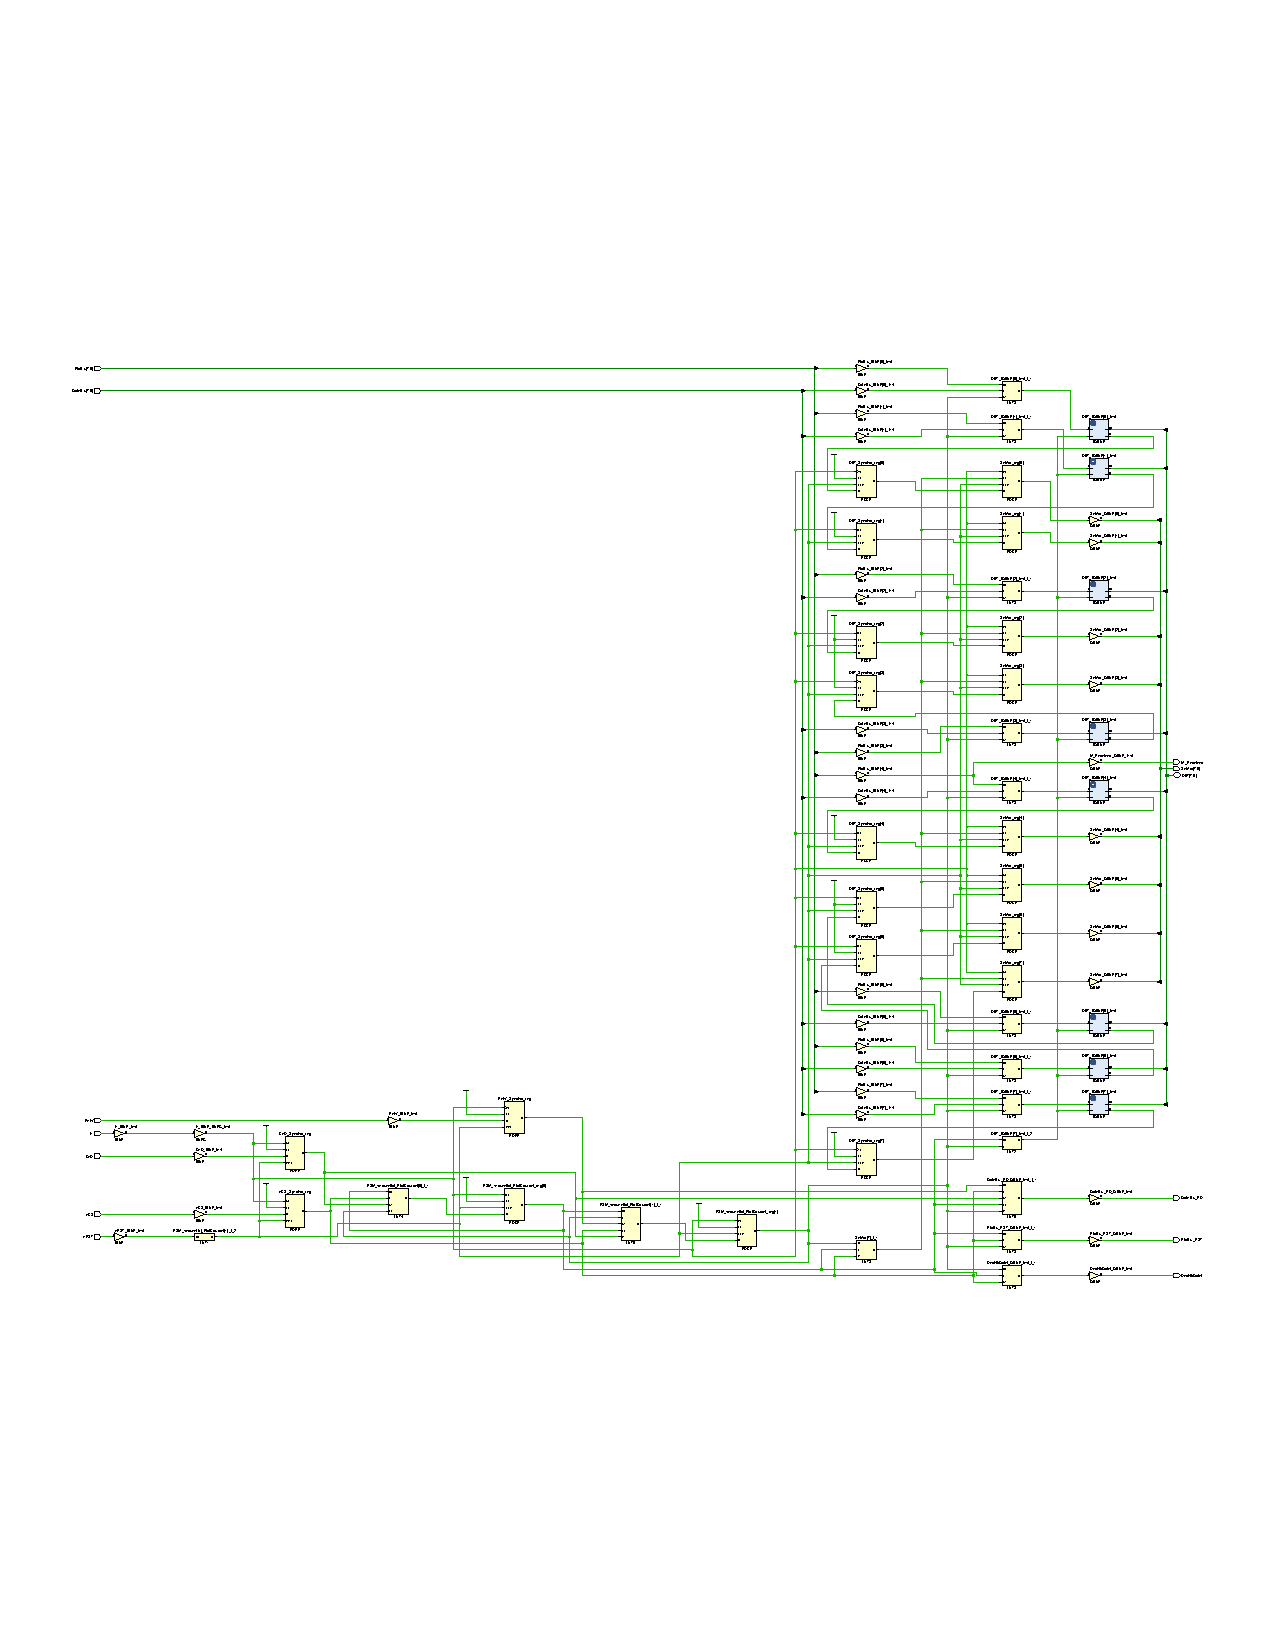
\includegraphics[width=0.8\linewidth]{images/Routage/schematic_RTL_VIVADO_recadre.pdf}
    \caption{Synthèse matérielle Vivado}
    \label{fig:rout_general}
\end{figure}

Cette synthèse nous montre que la logique est transformée en ressource matérielle, notamment des 
LUT (Look-Up Tables) et des Flip-Flops, qui sont les éléments de base pour implémenter la logique 
dans un FPGA.
\newline

Les \textbf{LUT} (Look-Up Tables), éléments fondamentaux d'un FPGA, peuvent être considérées comme 
des portes logiques programmables capables de réaliser toute fonction combinatoire. 
Elles constituent la base de l'implémentation matérielle et offrent une vision schématique complète 
du système.  
\newline

Prenons l'exemple d'une \textbf{LUT3} :  

\begin{figure}[H]
    \centering
    % Première image
    \begin{subfigure}[b]{0.55\linewidth}
        \centering
        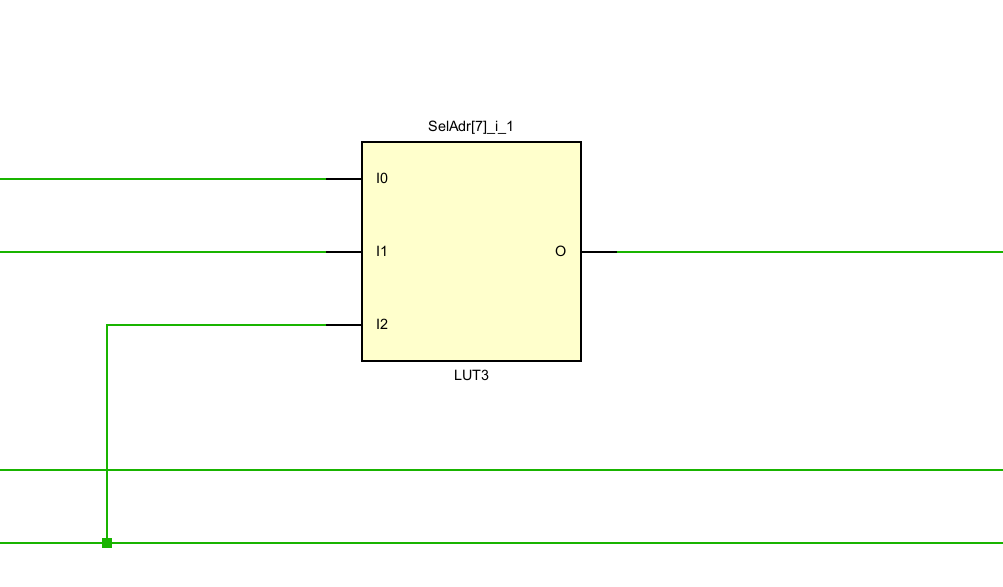
\includegraphics[width=\linewidth]{images/Routage/LUT_EXEMPLE.png}
        \caption{Exemple de LUT}
        \label{fig:lut_exemple}
    \end{subfigure}
    \hfill
    % Deuxième image
    \begin{subfigure}[b]{0.25\linewidth}
        \centering
        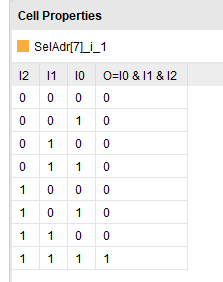
\includegraphics[width=\linewidth]{images/Routage/TABLE_LUT.png}
        \caption{Table de vérité associée}
        \label{fig:table_lut}
    \end{subfigure}
    \caption{Illustration d'une LUT et de sa table de vérité}
    \label{fig:lut_complete}
\end{figure}

Grace à la table de vérité de la LUT nous remarquons que cette LUT3 implémente une fonction logique ET à trois entrées.
\newline

\begin{figure}[H]
    \centering
    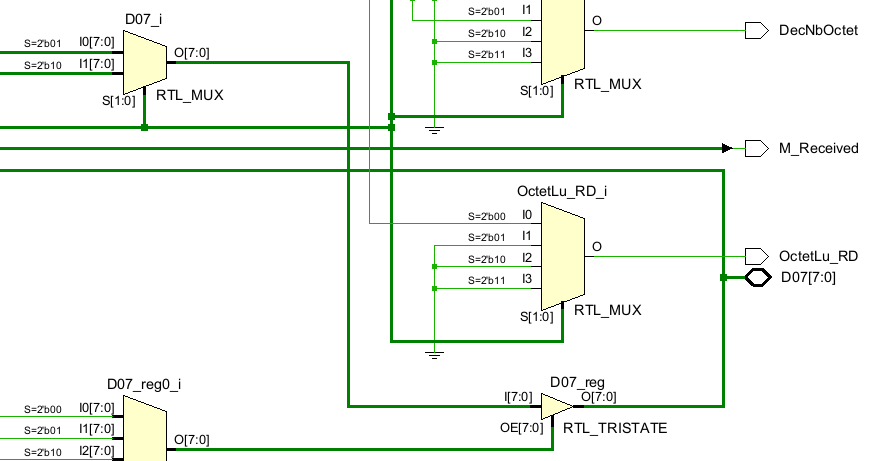
\includegraphics[width=0.8\linewidth]{images/Routage/Mux_Tris_Vivado.png}
    \caption{Synthèse Logique Vivado}
    \label{fig:rout_general}
\end{figure}

Nous observons également la présence de la partie opérative de l'interface Microprocesseur.
\newline

\medskip

La suite du flot de conception consiste à lancer l'\textbf{implémentation} du système afin d'obtenir le routage complet. 
Vivado propose alors une vue générale du FPGA, mettant en évidence ses différentes zones fonctionnelles :  

\begin{figure}[H]
    \centering
    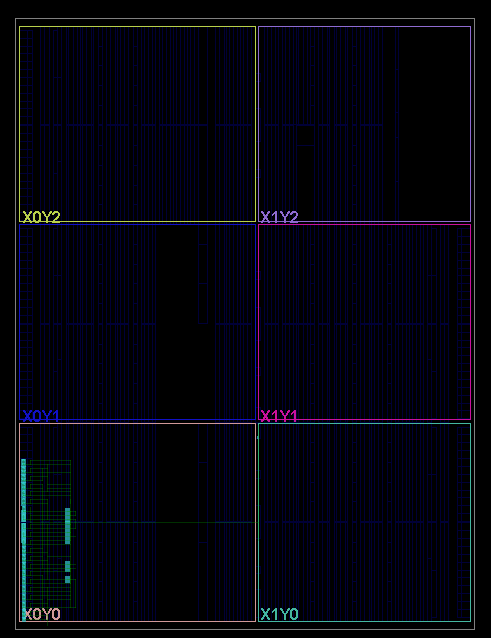
\includegraphics[width=0.8\linewidth]{images/Routage/Rout_1.png}
    \caption{Slice du FPGA après routage}
    \label{fig:rout_general}
\end{figure}

En effectuant un zoom, il est possible de constater que le système a été implémenté dans la zone \textbf{0} du FPGA. 
Nous observons que la zone située à gauche correspond aux entrées de chaque variable, 
celles-ci étant toutes reliées à des \textbf{buffers}.

\begin{figure}[H]
    \centering
    % Première image (anciennement deuxième)
    \begin{subfigure}[b]{0.45\linewidth}
        \centering
        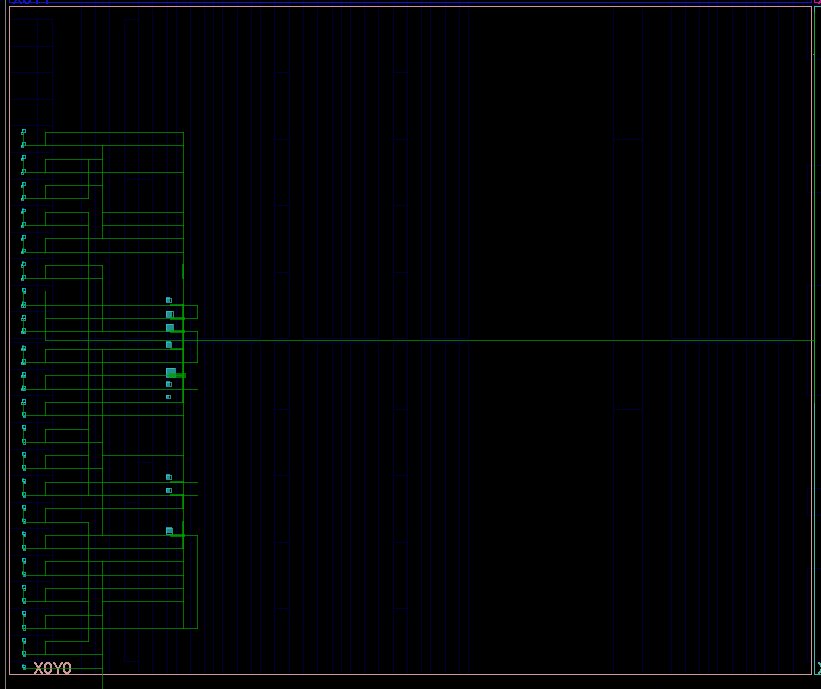
\includegraphics[width=\linewidth]{images/Routage/Rout_2.png}
        \caption{Localisation du système dans la zone 0 du FPGA}
        \label{fig:rout_zone0}
    \end{subfigure}
    \hfill
    % Deuxième image (anciennement première)
    \begin{subfigure}[b]{0.50\linewidth}
        \centering
        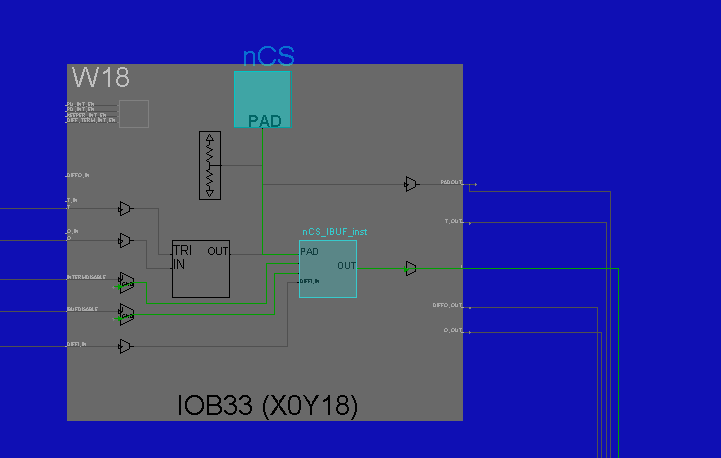
\includegraphics[width=\linewidth]{images/Routage/buff.png}
        \caption{Buffer associé à nCS}
        \label{fig:buff_ncs}
    \end{subfigure}
    \caption{Vue du système routé et des buffers associés sur le FPGA}
    \label{fig:rout_buff}
\end{figure}



Un zoom encore plus détaillé permet d'observer le câblage interne des ressources identifiées lors de la synthèse.  
Par exemple, une \textbf{LUT3} est câblée de la manière suivante :  

\begin{figure}[H]
    \centering
    % Première image
    \begin{subfigure}[b]{0.35\linewidth}
        \centering
        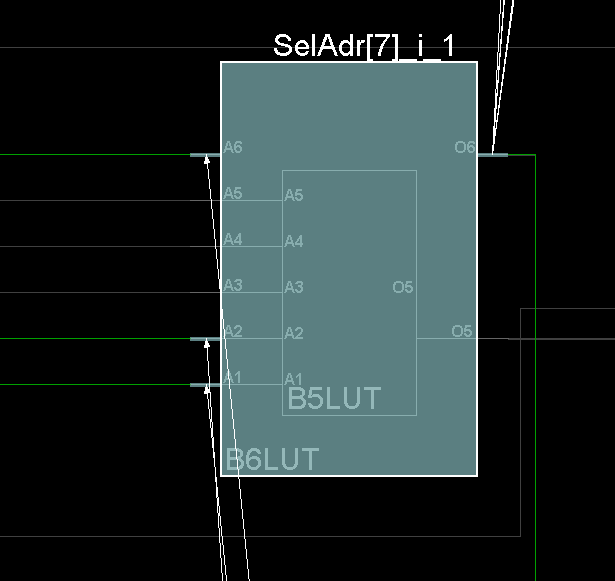
\includegraphics[width=\linewidth]{images/Routage/Rou_3.png}
        \caption{Connexion interne d'une LUT3}
        \label{fig:rout_lut3a}
    \end{subfigure}
    \hfill
    % Deuxième image
    \begin{subfigure}[b]{0.55\linewidth}
        \centering
        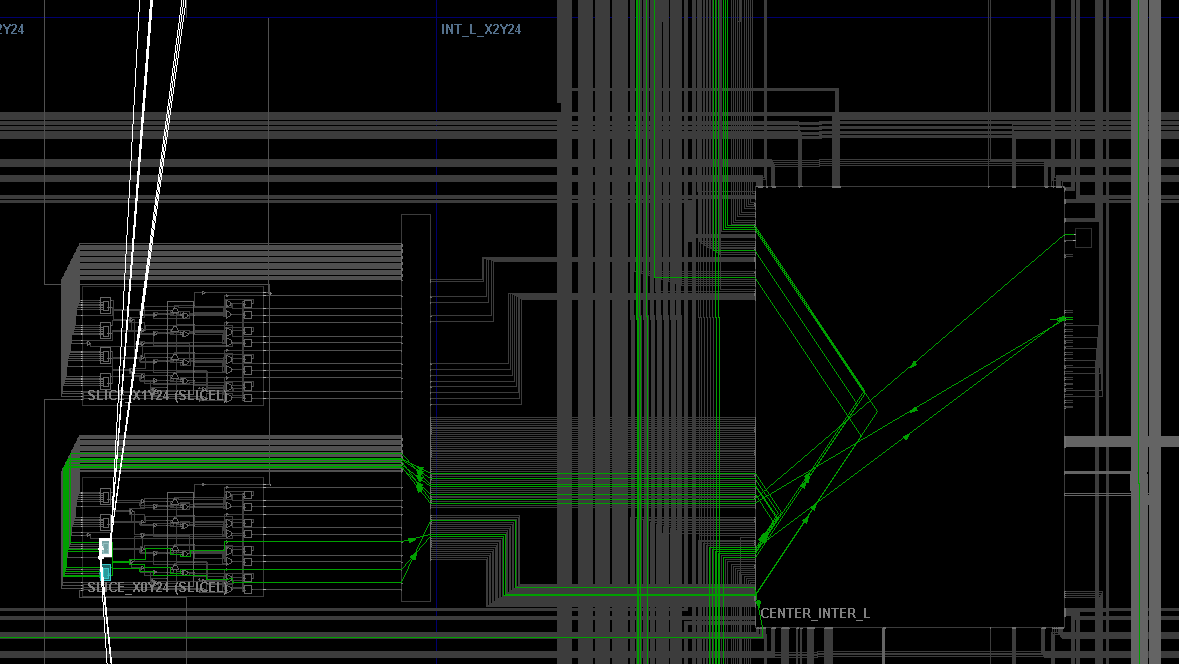
\includegraphics[width=\linewidth]{images/Routage/Rou_4.png}
        \caption{Schéma détaillé du câblage LUT3}
        \label{fig:rout_lut3b}
    \end{subfigure}
    \caption{Exemple de routage d'une LUT3 dans le FPGA}
    \label{fig:rout_lut3}
\end{figure}

\medskip

Le résultat final est une représentation complète et hiérarchisée du système, directement mappée sur le FPGA. 
\textbf{Vivado} offre ainsi la possibilité de visualiser l'ensemble du flot, depuis la description logique RTL jusqu'au routage physique détaillé.  

En résumé, la conception suit une progression en trois étapes :  
\begin{itemize}
    \item la \textbf{synthèse} génère une description logique optimisée du système (LUT, registres, blocs fonctionnels) ;  
    \item le \textbf{placement} attribue ces ressources aux cellules physiques du FPGA ;  
    \item le \textbf{routage} établit les interconnexions nécessaires au bon fonctionnement du circuit.  
\end{itemize}

Cette approche permet de passer d'une description abstraite en langage HDL à une implémentation matérielle 
concrète, où chaque fonction logique est traduite en ressources physiques. 
Vivado fournit alors une vision globale et détaillée du FPGA, allant de la logique combinatoire jusqu'au câblage interne des composants.


\section{Conclusion}

Pour ce premier rapport concernant le projet \textbf{Réception LIN} de conception de circuit numérique, 
nous avons suivi plusieurs étapes successives afin de concevoir ce système.  

Dans un premier temps, lors des séances de TD, nous avons décomposé notre étude en plusieurs parties afin de répondre au cahier des charges. 
L’utilisation du \textbf{diagramme en Y} nous a permis d’analyser séparément chacune de ces étapes et de structurer notre démarche. 
\newline

La phase de \textbf{spécification fonctionnelle} nous a permis de définir l’ensemble des ressources 
nécessaires, 
en lien direct avec le cahier des charges, ainsi que le nombre de blocs et les signaux de base.  
\newline

Ensuite, la \textbf{solution architecturale} a permis de préciser chaque partie en les reliant à des 
modèles connus 
(machines séquentielles, machines de Moore ou machines de Mealy). 
Cette étape a été essentielle pour découper notre système en une partie opérative et une partie commande :  
\newline

\begin{itemize}
    \item la partie opérative a été conçue à partir de blocs logiques simples (multiplexeurs, bascules D, etc.) ;  
    \item la partie commande a été décrite sous forme d’automates, associés à des machines de Moore ou de Mealy, 
    afin d’obtenir une description claire et structurée.  
\end{itemize}
Cette méthodologie nous a permis d’écrire un code plus simple, lisible et cohérent.  

La phase de \textbf{simulation} a ensuite validé le fonctionnement du système en stimulant les différents ports d’entrée 
et en observant les sorties.  
\newline

La phase de \textbf{synthèse} nous a permis de vérifier la logique interne du système à travers les schémas RTL générés. 
Ces schémas ont ensuite été exploités dans Vivado, qui a associé les différentes fonctions logiques aux \textbf{LUT}.  
\newline

Enfin, l’\textbf{implémentation} nous a donné accès au routage sur FPGA. 
Cette étape a permis de vérifier concrètement l’affectation des ressources matérielles et le câblage interne du système.  
\newline

En conclusion, ce premier travail nous a permis de valider l’\textbf{interface microprocesseur}. 
La suite du projet consistera à finaliser la conception complète du récepteur LIN afin de répondre à l’intégralité du cahier des charges.


\section{Annexes}

\subsection{Testbench InterfaceMicroprocesseur}

\begin{lstlisting}[style=VHDLStyle, caption={Testbench InterfaceMicroprocesseur}]
LIBRARY ieee;
USE ieee.std_logic_1164.all;
USE ieee.std_logic_arith.all;

ENTITY EnvTest_InterfaceMicroprocesseur IS
   GENERIC( 
      CLOCK_PERIOD   : time := 50 ns;
      RESET_OFFSET   : time := 500 ns;
      RESET_DURATION : time := 300 ns;
      ACCESS_TIME    : time := 40 ns;
      HOLD_TIME      : time := 70 ns
   );
   PORT( 
      M_Received : IN     std_logic;
      CnD        : OUT    std_logic;
      H          : OUT    std_logic;
      RnW        : OUT    std_logic;
      nCS        : OUT    std_logic;
      nRST       : OUT    std_logic;
      D07        : INOUT  std_logic_vector (7 DOWNTO 0)
   );
-- Declarations

END EnvTest_InterfaceMicroprocesseur ;

--
ARCHITECTURE arch OF EnvTest_InterfaceMicroprocesseur IS
TYPE DefState IS (Waiting, DataReading, StateReading, FilterWriting);

SIGNAL ProcessorState : DefState;

BEGIN
  
ClockGeneratorProc : PROCESS
BEGIN
  H <= '0';
  WAIT FOR CLOCK_PERIOD/2;
  H <= '1';
  WAIT FOR CLOCK_PERIOD/2;
END PROCESS ClockGeneratorProc;

ResetGeneratorProc : PROCESS
BEGIN
  nRST <= '1';
  WAIT FOR RESET_OFFSET;
  nRST <= '0';
  WAIT FOR RESET_DURATION;
  nRST <= '1';
  WAIT;
END PROCESS ResetGeneratorProc;

ProcessorBehaviorProc : PROCESS
BEGIN
  D07 <= (others => 'Z');
--Waiting cycle--
  ProcessorState <= Waiting;
  nCS <= '1';
  CnD <= '1';
  RnW <= '1';
  WAIT FOR RESET_OFFSET+RESET_DURATION+2*CLOCK_PERIOD;    
--Reading data cycle--
  ProcessorState <= DataReading;
  WAIT FOR ACCESS_TIME;
  nCS <= '0';
  CnD <= '0';
  RnW <= '1';
  WAIT FOR 2*CLOCK_PERIOD;
--Waiting cycle--
  ProcessorState <= Waiting;
  nCS <= '1'; 
  CnD <= '1';
  RnW <= '1';
  WAIT FOR 2*CLOCK_PERIOD-ACCESS_TIME;
--Reading state cycle--
  ProcessorState <= StateReading;
  WAIT FOR ACCESS_TIME;
  nCS <= '0';
  CnD <= '1';
  RnW <= '1';
  WAIT FOR 2*CLOCK_PERIOD;
--Waiting cycle--
  ProcessorState <= Waiting;
  nCS <= '1';
  CnD <= '1';
  RnW <= '1';
  WAIT FOR 2*CLOCK_PERIOD-ACCESS_TIME;
--Writing cycle--
  ProcessorState <= FilterWriting;
  WAIT FOR ACCESS_TIME;
  nCS <= '0';
  CnD <= '0';
  RnW <= '0';
  D07 <= (others => '1');
  WAIT FOR 2*CLOCK_PERIOD;
--Waiting cycle--
  ProcessorState <= Waiting;
  nCS <= '1';
  CnD <= '1';
  RnW <= '1';
  WAIT FOR HOLD_TIME;
  D07 <= (others => 'Z');
  WAIT;
END PROCESS ProcessorBehaviorProc;

END ARCHITECTURE arch;

\end{lstlisting}

\listoffigures

\end{document}